\documentclass[10pt]{beamer}
\usetheme[progressbar=frametitle]{m}
\usepackage[frenchb]{babel}
\usepackage[utf8]{inputenc}
\usepackage{soul}

\usepackage{booktabs}
\usepackage[scale=2]{ccicons}

\usepackage{pgfplots}
\usepgfplotslibrary{dateplot}

\usepackage{pdfpages}
\usepackage{hyperref}
\usepackage{listings}
\usepackage{color}
\usepackage{graphicx}
\usepackage{amsmath}
\usepackage{movie15}
\usepackage[upright]{fourier}
\usepackage{pgfpages}

%\setbeameroption{show notes on second screen=right}

\title{\textbf{\LARGE{Raytracer,}}\\\bigskip\texttt{\small{~~Projection de formes 4D\\~~~~~~~~dans un espace 3D\\~~~...~sur votre écran 2D.}}}
\author{\textsc{Baché} Antoine\\\textsc{Petrenko} Ludovic\\\textsc{Arnaud} Arthur\\\textsc{Boulagnon} Luka}
\date{\today}

\begin{document}

\begin{frame}[fragile]
	\titlepage
\end{frame}

\plain{\pause \texttt{Projections, \pause \textit{ray-casting}, \pause et \textit{ray-tracing}.}%
\note[item]{Projection correspond au dessin, dans dimensn, d'1 forme en dimensn différente}%
\note[item]{Raycasting = }%
\note[item]{Raytracing = projeter 1 rayon pr 1 point de l'image 2D dans espace 3D}}

\begin{frame}[fragile]{Sommaire}
	\only<2->{\tableofcontents[pausesections]}
\end{frame}

\section{Rendering}

\begin{frame}[fragile]{Rendering \& optimisations}
	\begin{itemize}[<+->]
		\item Système de box pour chaque élément~;
		\item Système de partitionnement de l'espace~;
	\end{itemize}
\end{frame}

\begin{frame}[fragile]{Ray-tracing}
	\only<1>{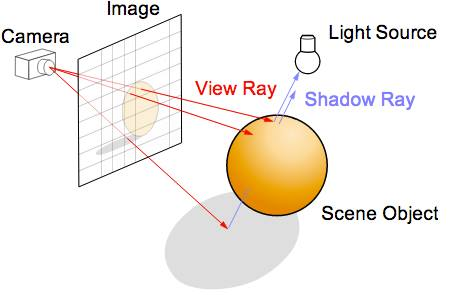
\includegraphics[width=9cm]{./imgs/ray-tracing.png}}
	\only<2>{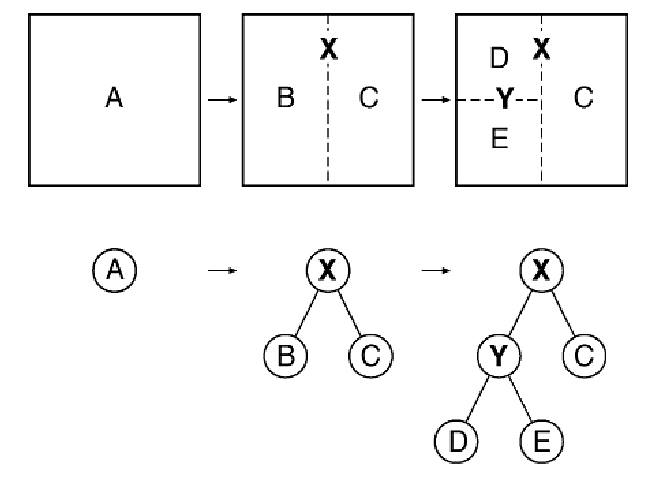
\includegraphics[width=9cm]{./imgs/bsp.png}}
\end{frame}

\subsection{Temps réel}

\begin{frame}[fragile]{En direct}
	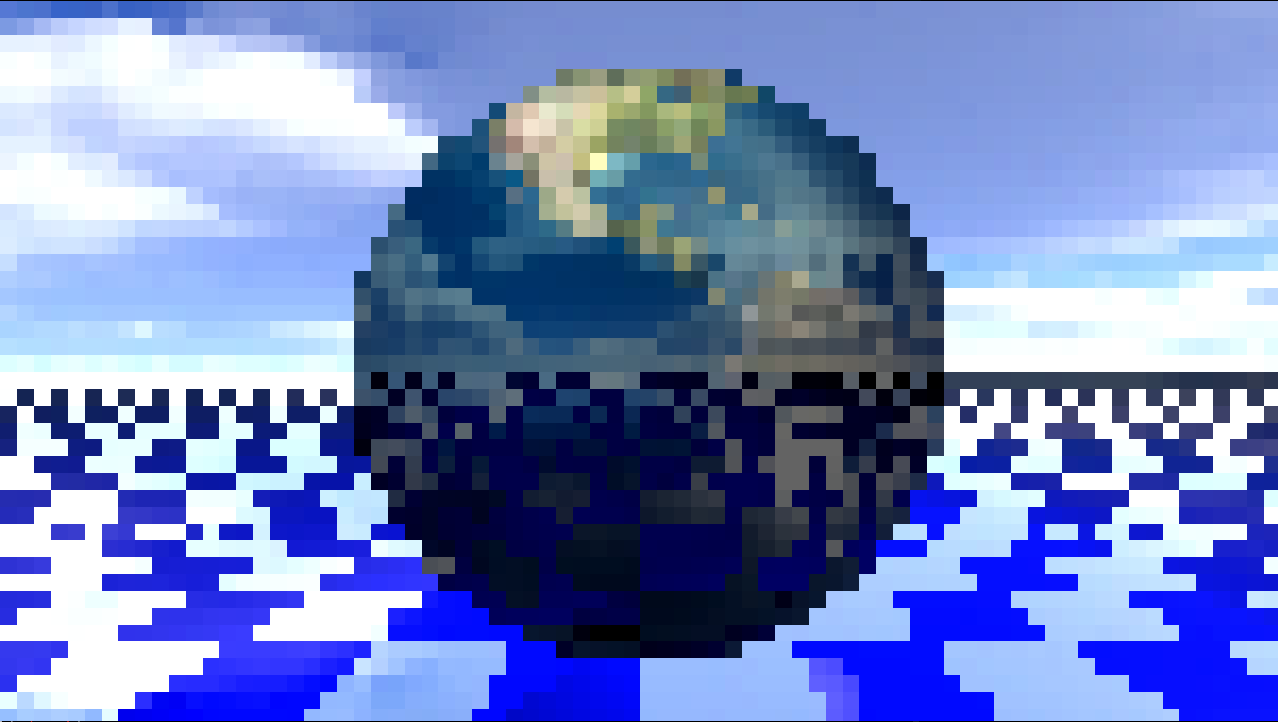
\includegraphics[width=9cm]{./imgs/live.png}
\end{frame}

\subsection{Rendu final}

\begin{frame}[fragile]{Rendu final}
	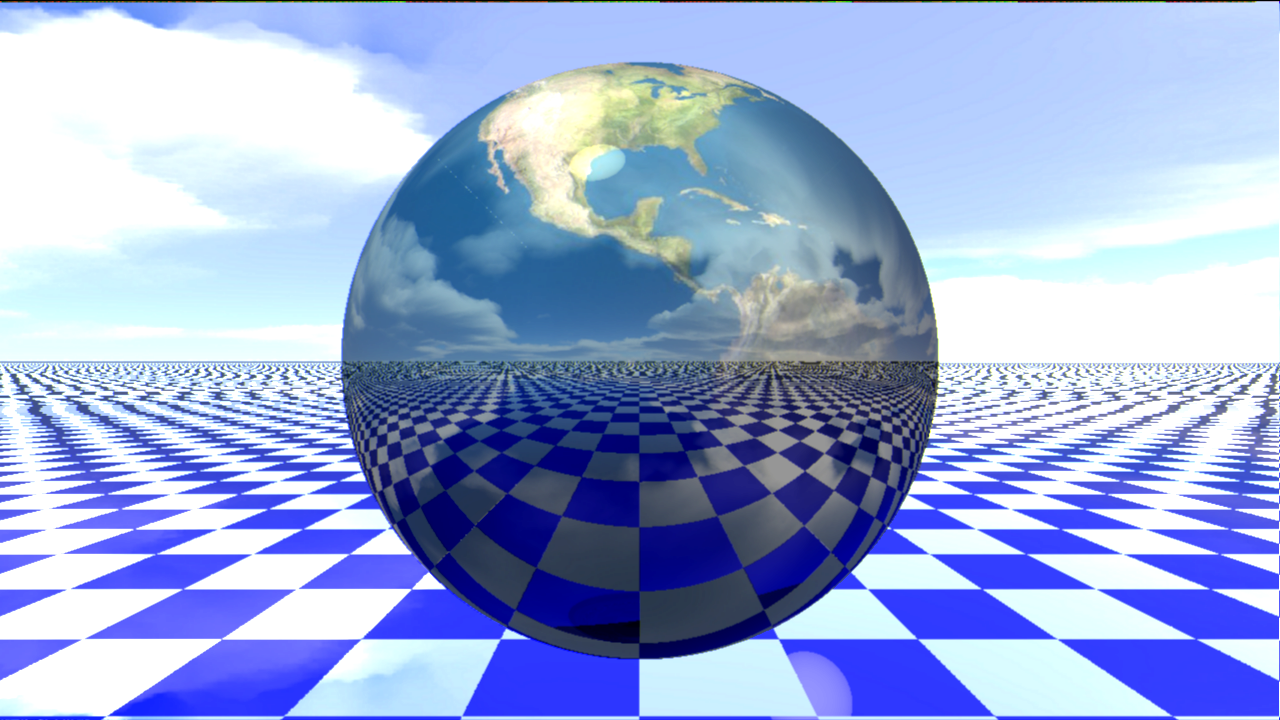
\includegraphics[width=9cm]{./imgs/sphere.png}
\end{frame}

\section{Techniquement}

\begin{frame}[fragile]{Thread pool}
	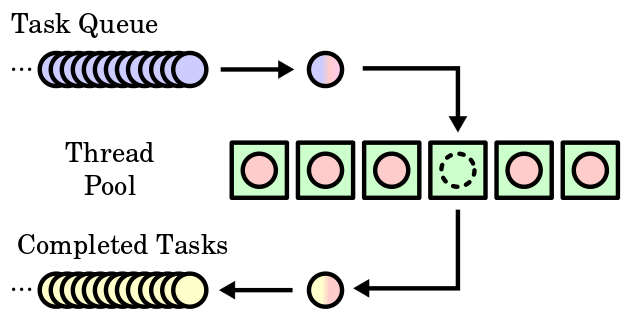
\includegraphics[width=9cm]{./imgs/thread_pool.png}
\end{frame}

\begin{frame}[fragile]{Gestion des formes}
	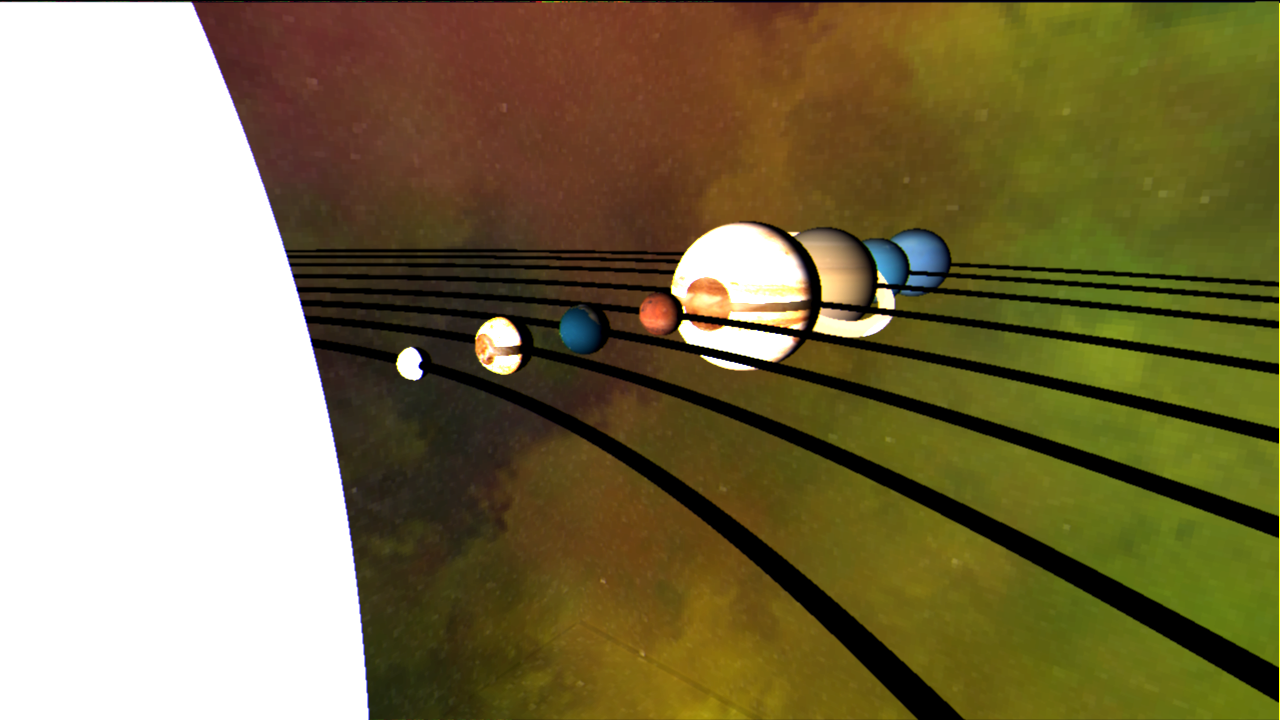
\includegraphics[width=9cm]{./imgs/solar.png}
	\pause
	\\
	\bigskip
	Tout l'ensemble du code a été pensé \og \textit{objet} \fg.
\end{frame}

\begin{frame}[fragile]{Ajout d'une nouvelle forme}
	Script de factorisation de l'équation des formes en fonction du degré d'équation~:

	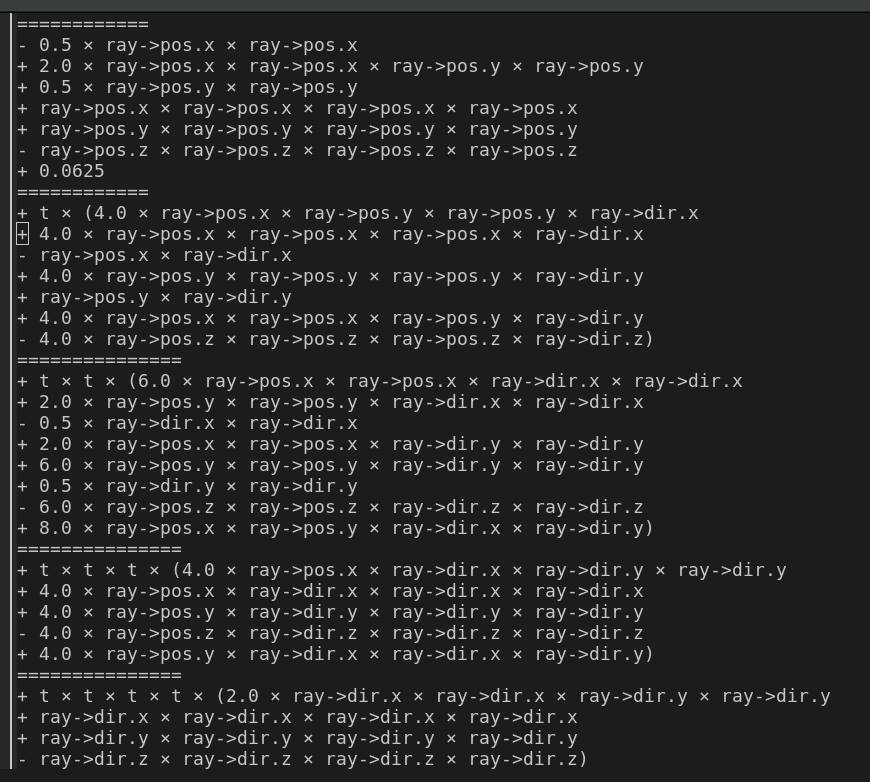
\includegraphics[height=6cm]{./imgs/toto.png}
\end{frame}

\section{Formes}

\begin{frame}[fragile,t,c]{Liste des formes}
	\only<1>{Sphère \& plan~:\\\bigskip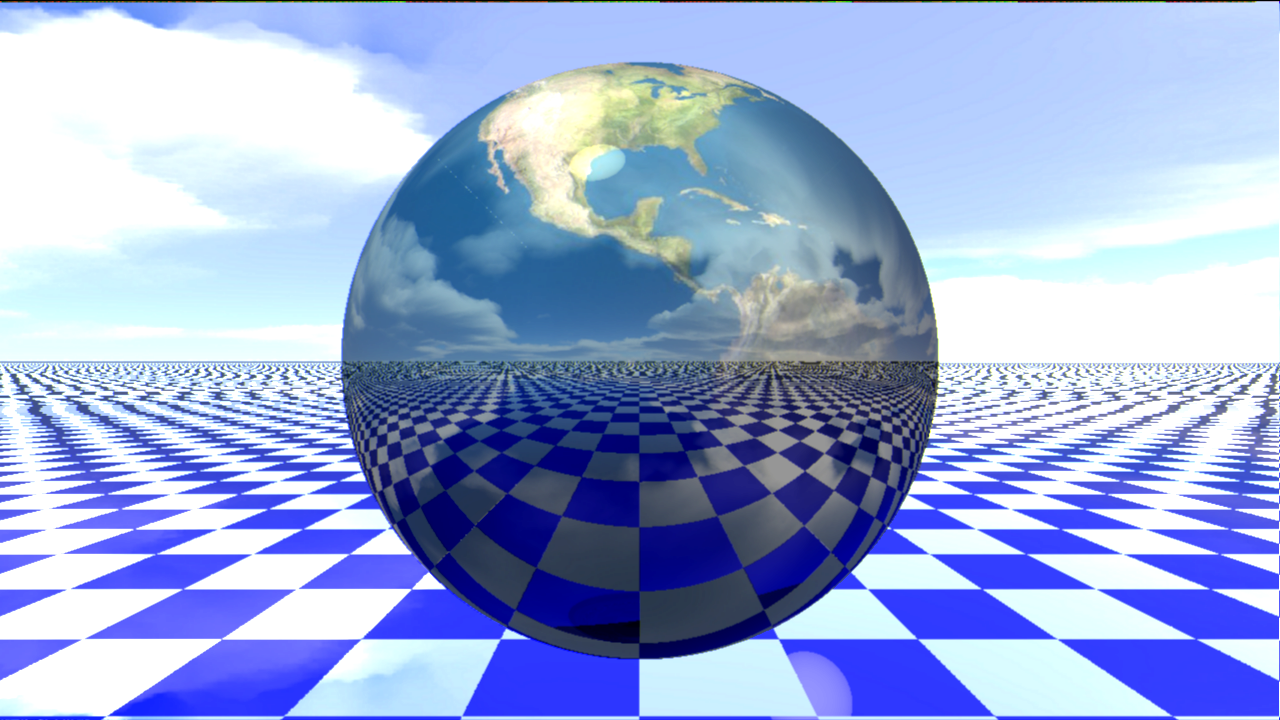
\includegraphics[width=9cm]{./imgs/sphere.png}}
	\only<2>{Cylindre~:\\\bigskip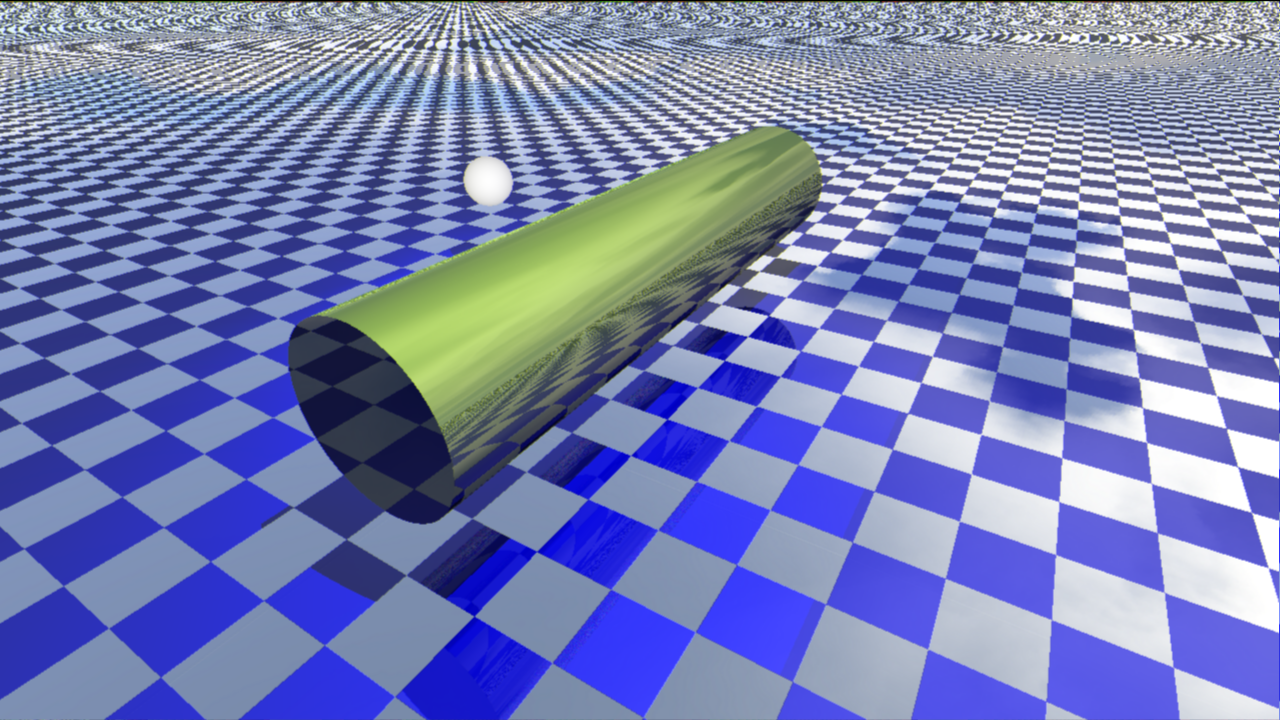
\includegraphics[width=9cm]{./imgs/cylinder.png}}
	\only<3>{Cône~:\\\bigskip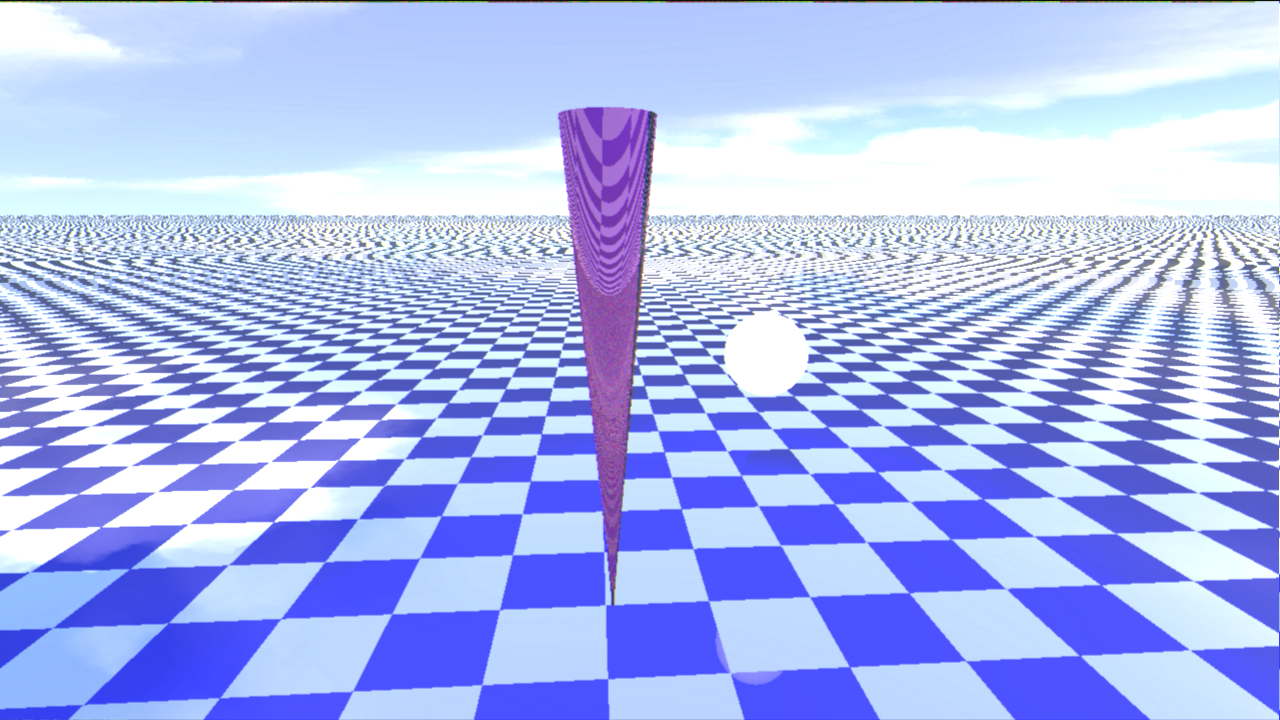
\includegraphics[width=9cm]{./imgs/cone.png}}
	\only<4>{Tore~:\\\bigskip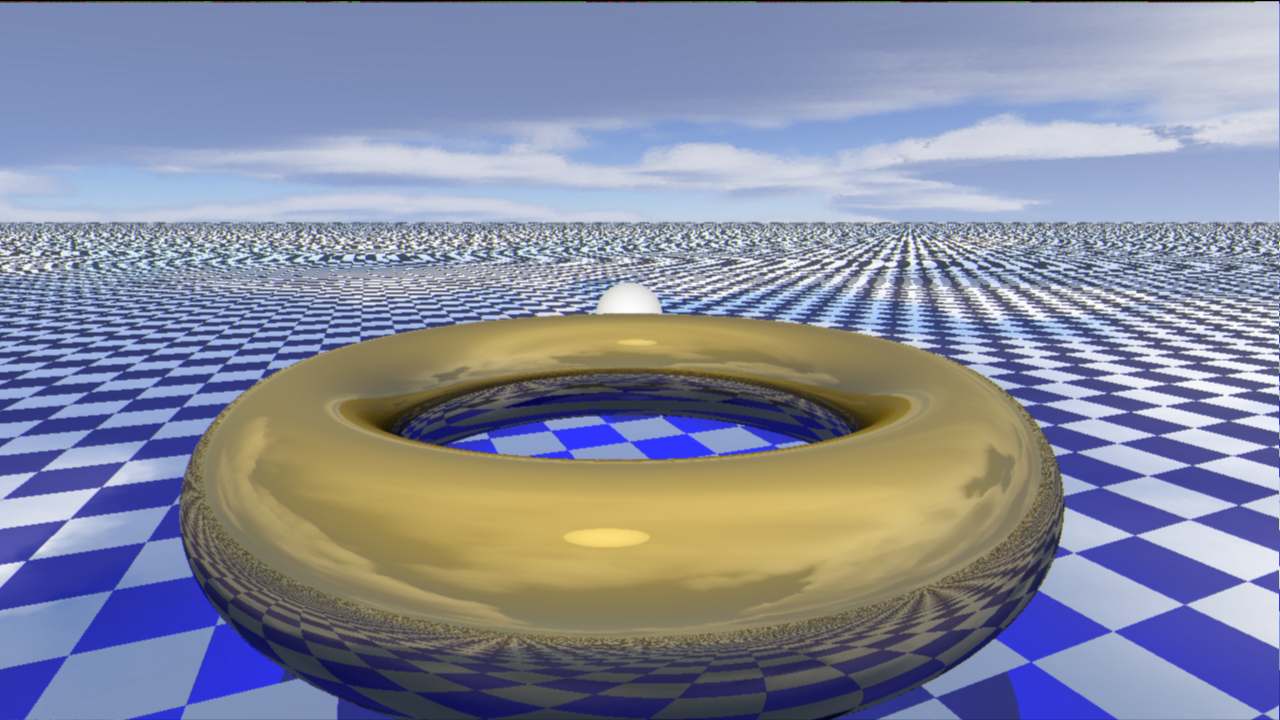
\includegraphics[width=9cm]{./imgs/torus.png}}
	\only<5>{Moëbius~:\\\bigskip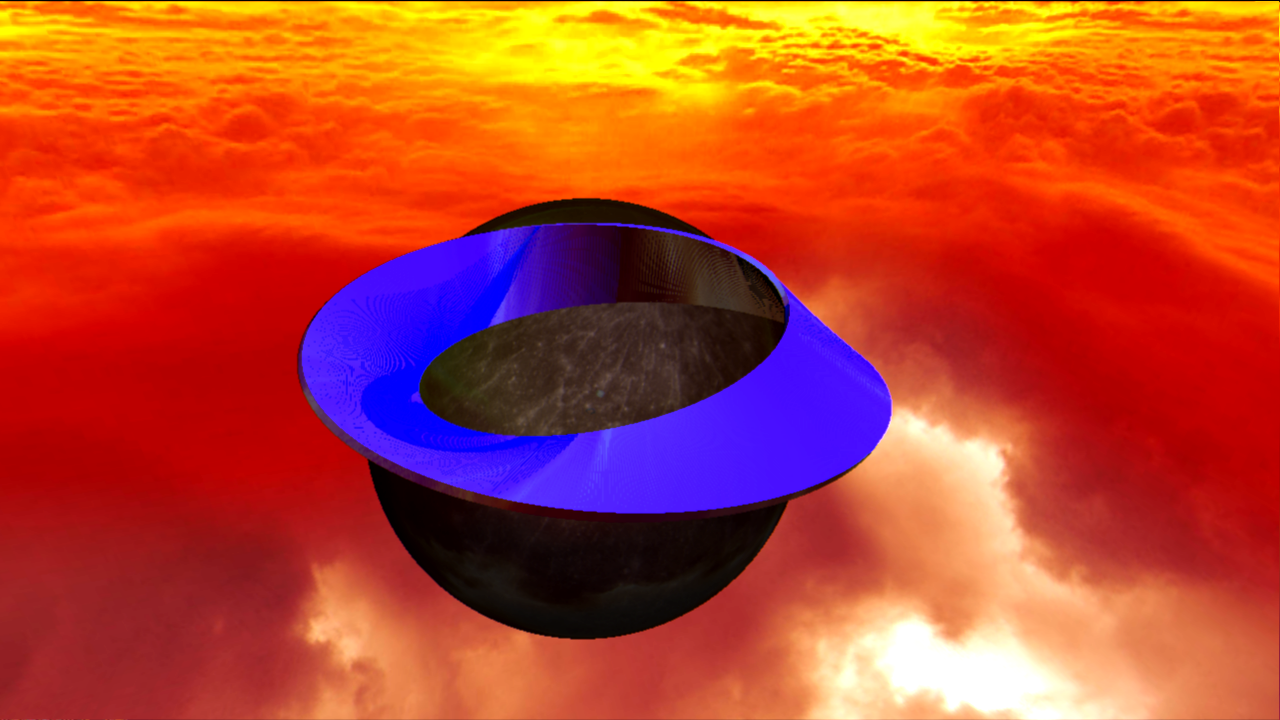
\includegraphics[width=9cm]{./imgs/mobius.png}}
	\only<6>{\textit{Void Cube}~:\\\bigskip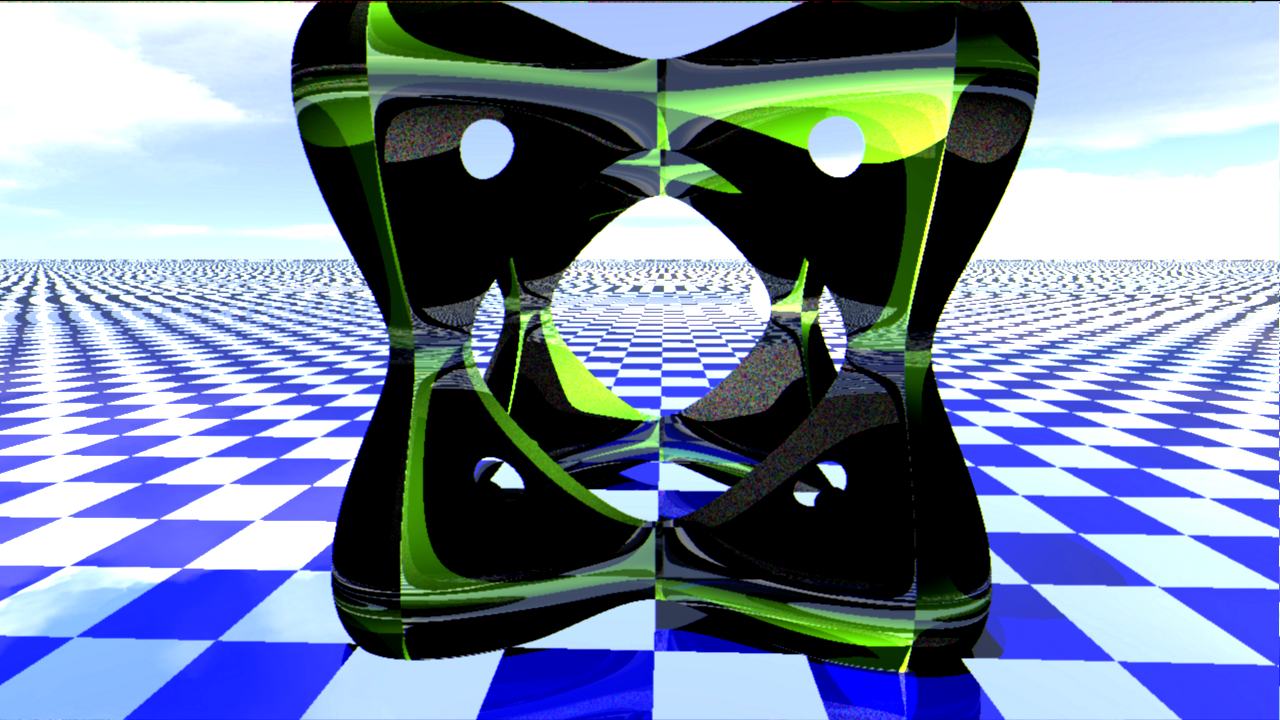
\includegraphics[width=9cm]{./imgs/void_cube.png}}
	\only<7>{Bouteille de Klein~:\\\bigskip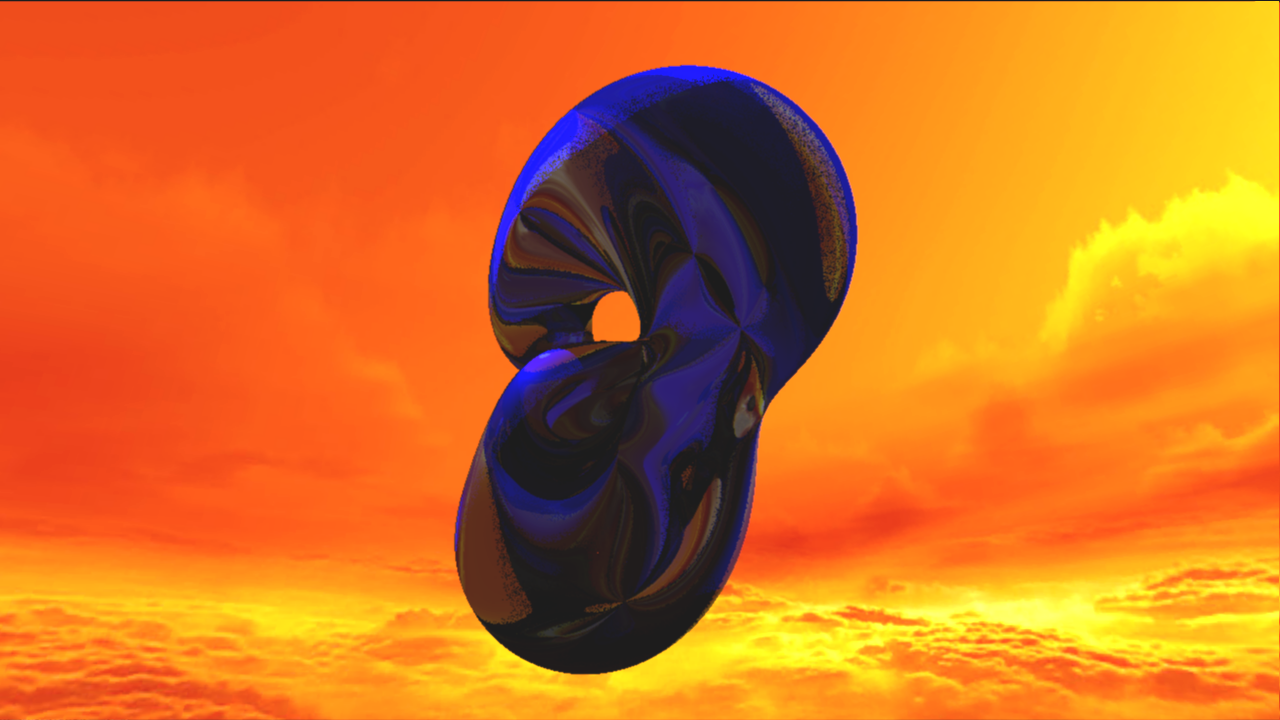
\includegraphics[width=9cm]{./imgs/klein.png}}
	\only<8>{\textit{Hyperbola}~:\\\bigskip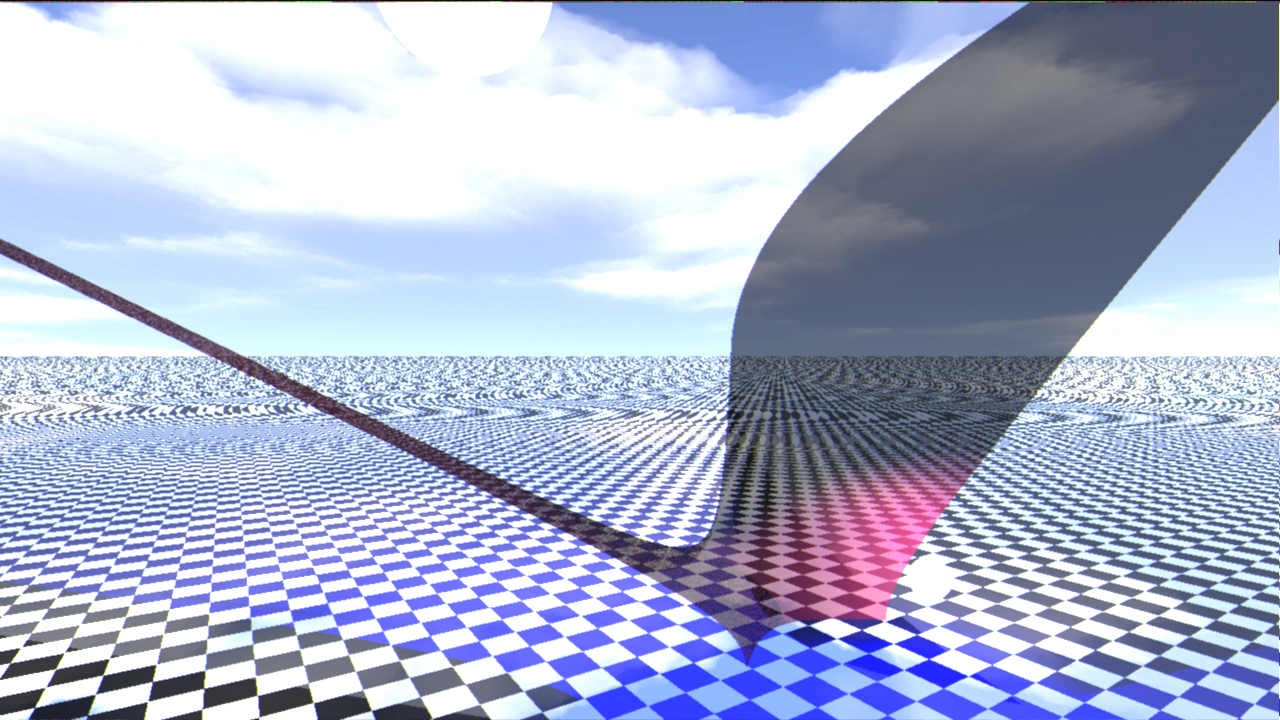
\includegraphics[width=9cm]{./imgs/hyperbola.png}}
	\only<9>{Ellipsoïde~:\\\bigskip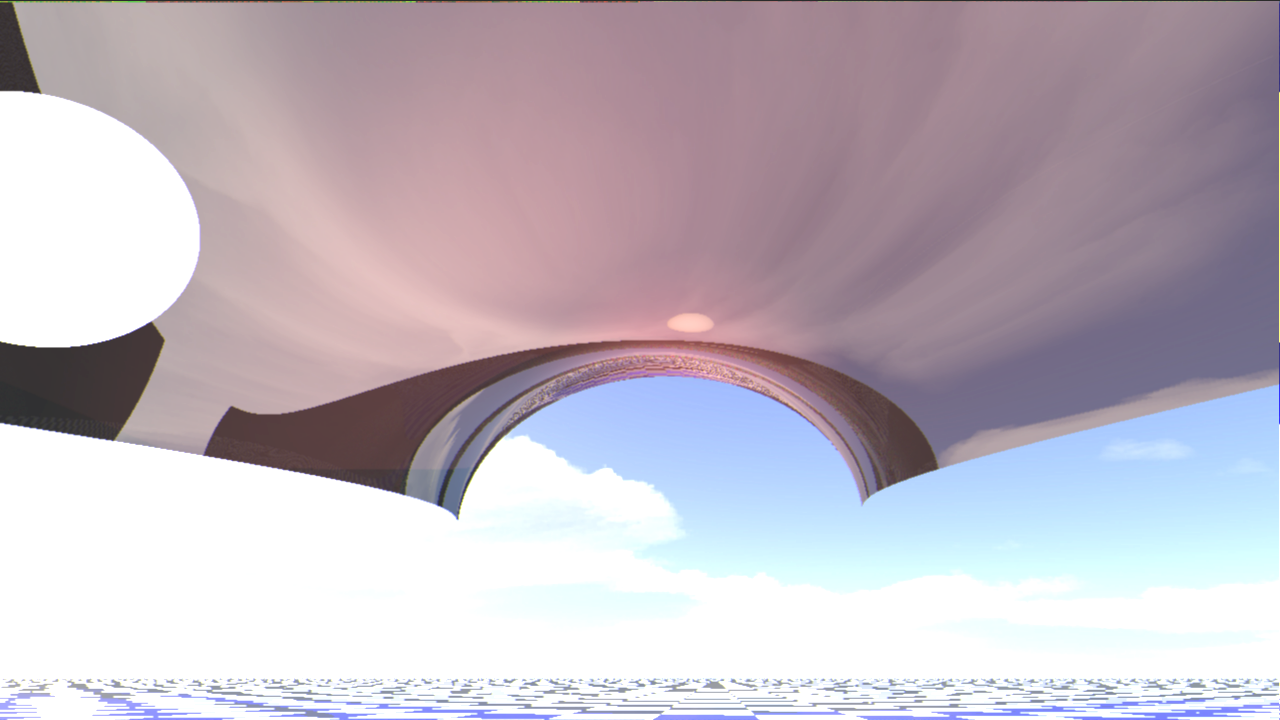
\includegraphics[width=9cm]{./imgs/ellipsoid.png}}
	\only<10>{Ovale de Cassini~:\\\bigskip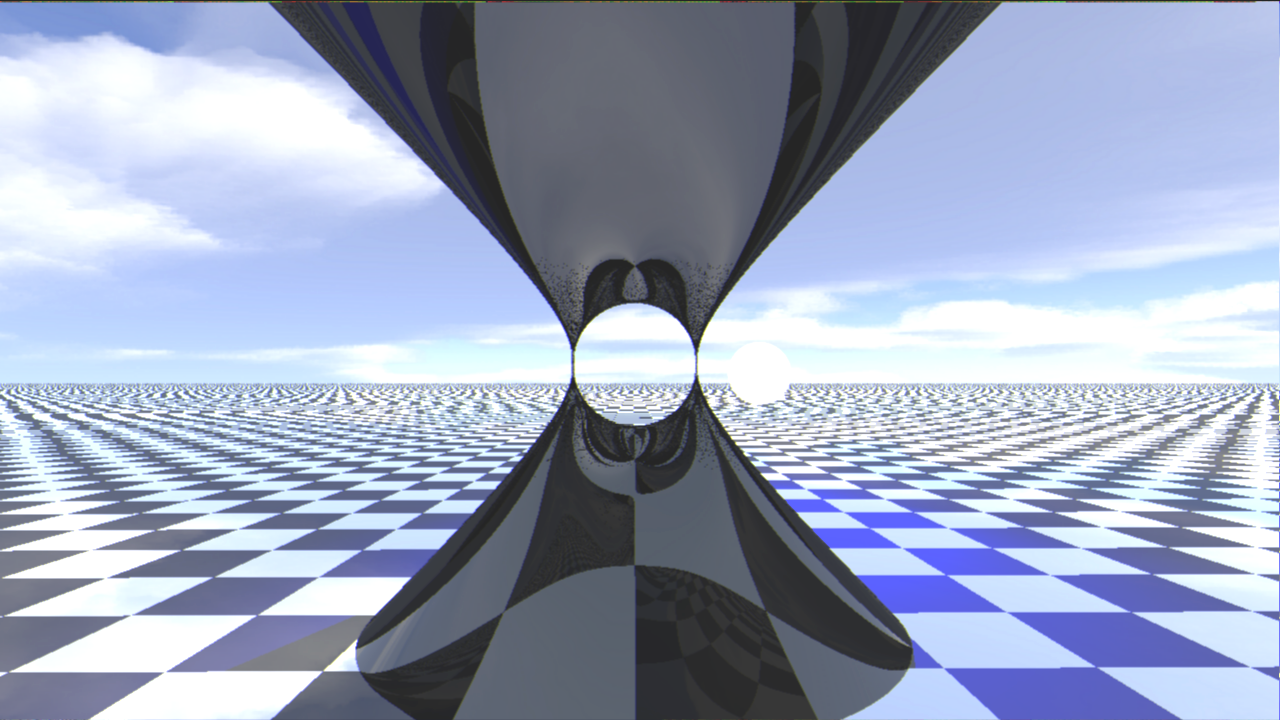
\includegraphics[width=9cm]{./imgs/cassini.png}}
	\only<11>{\textit{Chair}~:\\\bigskip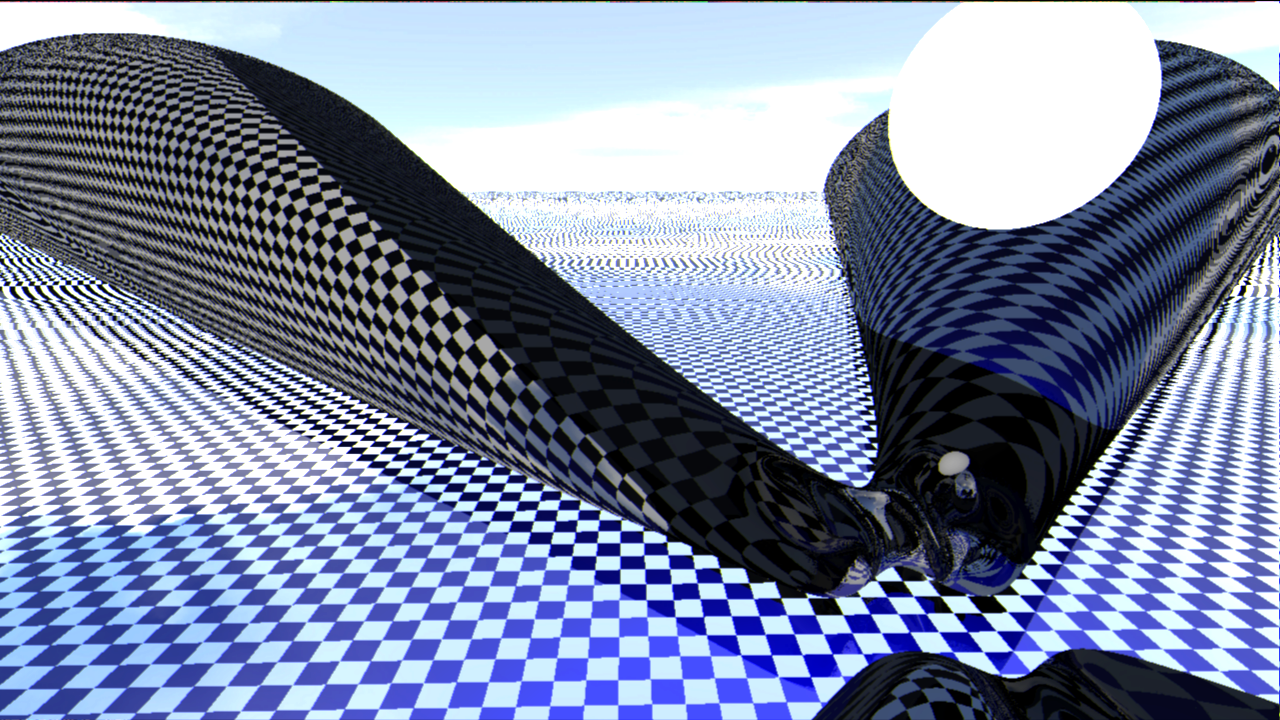
\includegraphics[width=9cm]{./imgs/chair.png}}
	\only<12>{\textit{Tetrahedral}~:\\\bigskip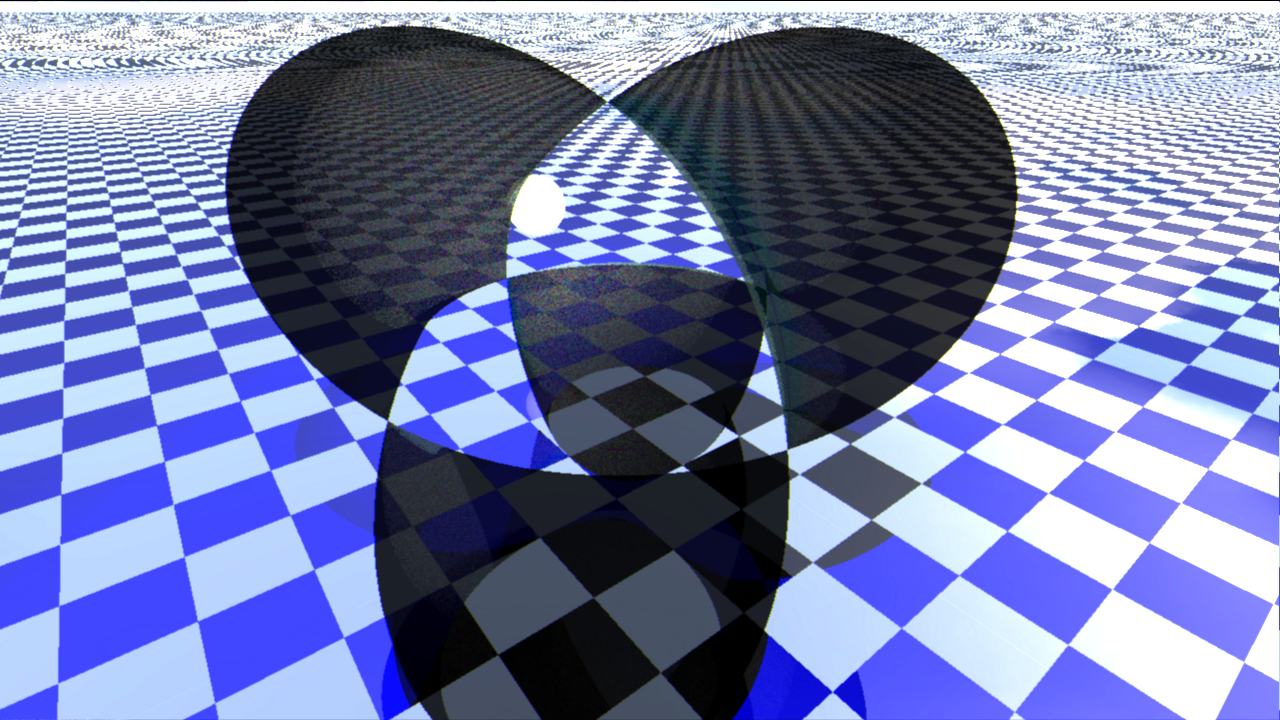
\includegraphics[width=9cm]{./imgs/tetrahedral.png}}
	\only<13>{\textit{Bifolia}~:\\\bigskip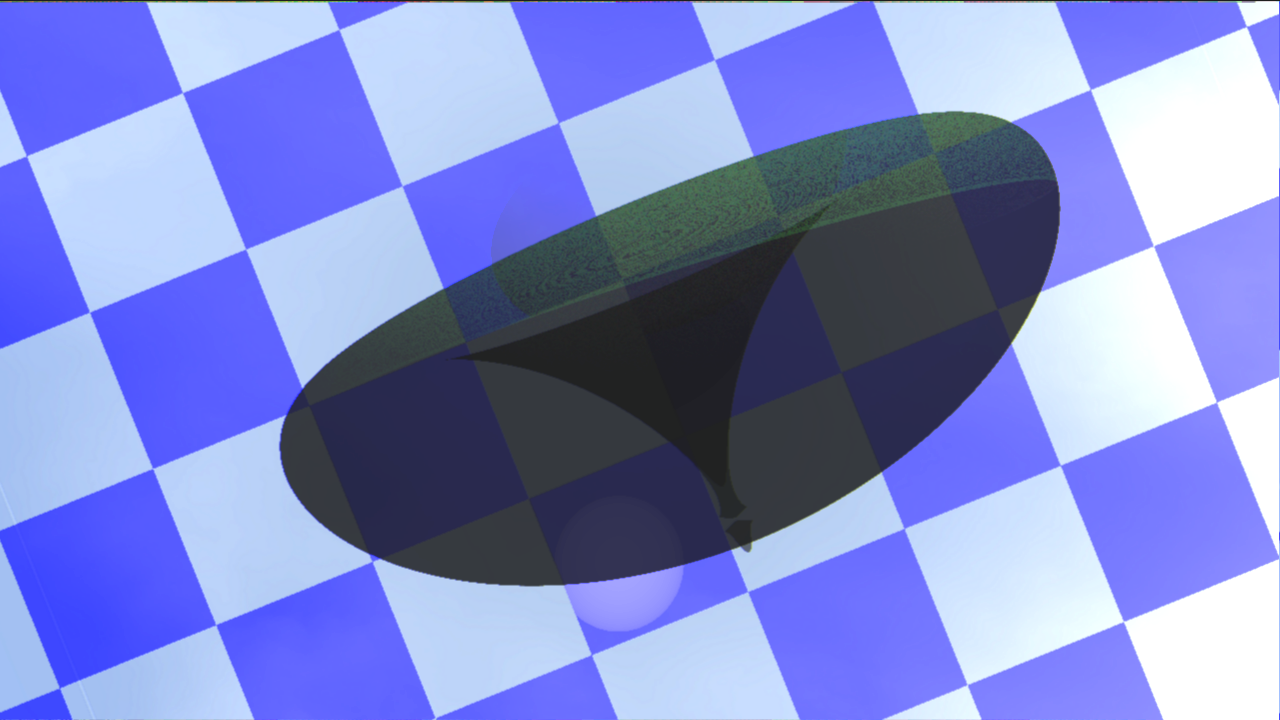
\includegraphics[width=9cm]{./imgs/bifolia.png}}
	\only<14>{\textit{Duplin}~:\\\bigskip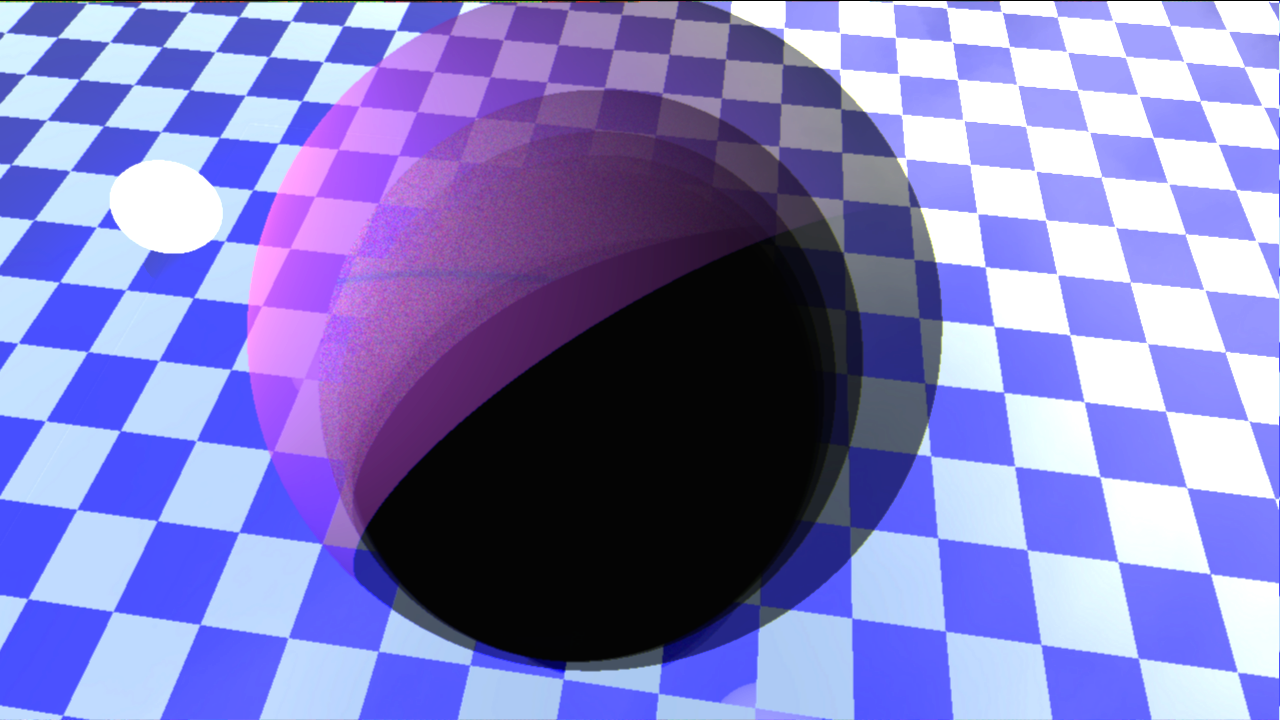
\includegraphics[width=9cm]{./imgs/duplin.png}}
	\only<15>{\textit{Cushion}~:\\\bigskip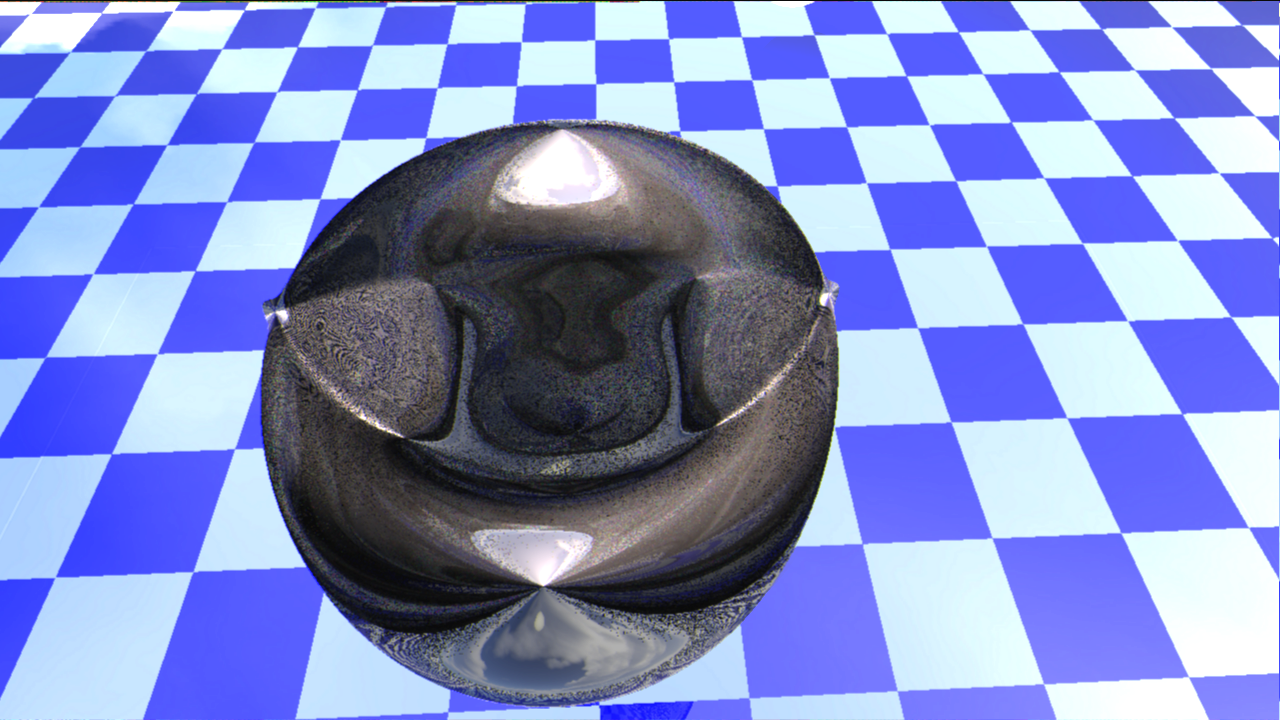
\includegraphics[width=9cm]{./imgs/cushion.png}}
	\only<16>{\textit{Tooth}~:\\\bigskip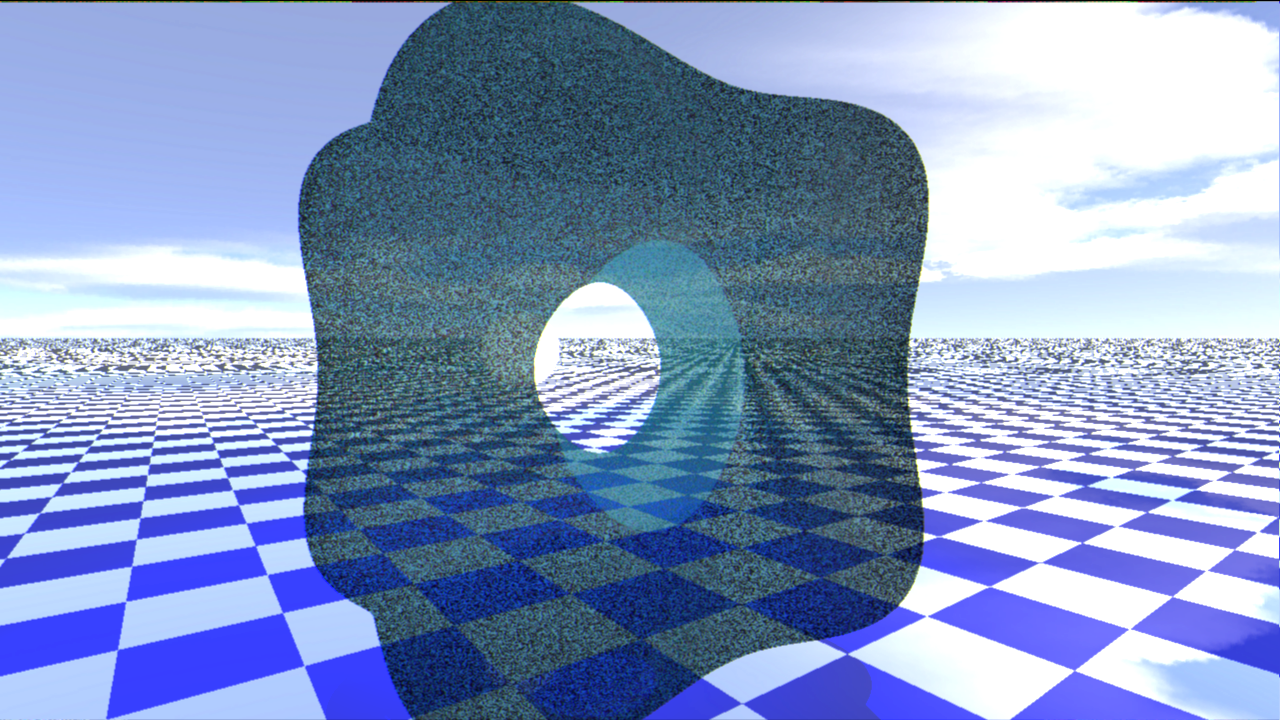
\includegraphics[width=9cm]{./imgs/tooth.png}}
	\only<17>{\textit{Hunt}~:\\\bigskip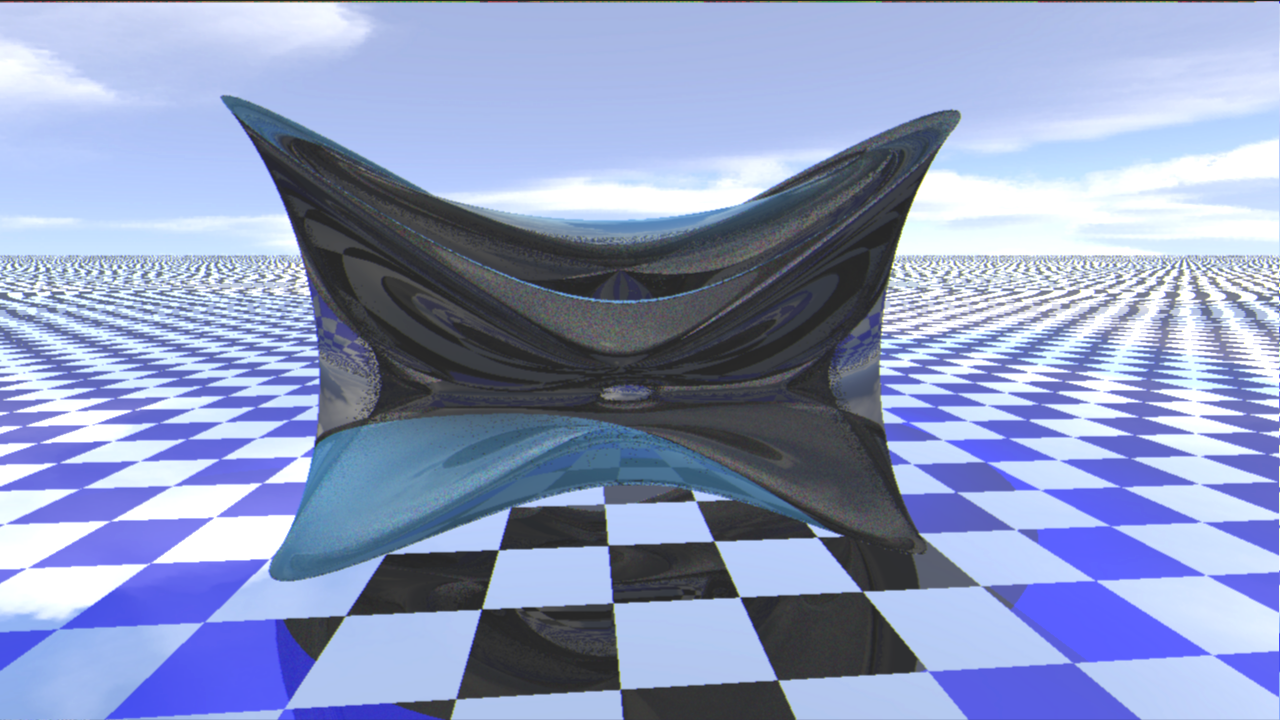
\includegraphics[width=9cm]{./imgs/hunt.png}}
	\only<18>{\textit{Bohemian Dome}~:\\\bigskip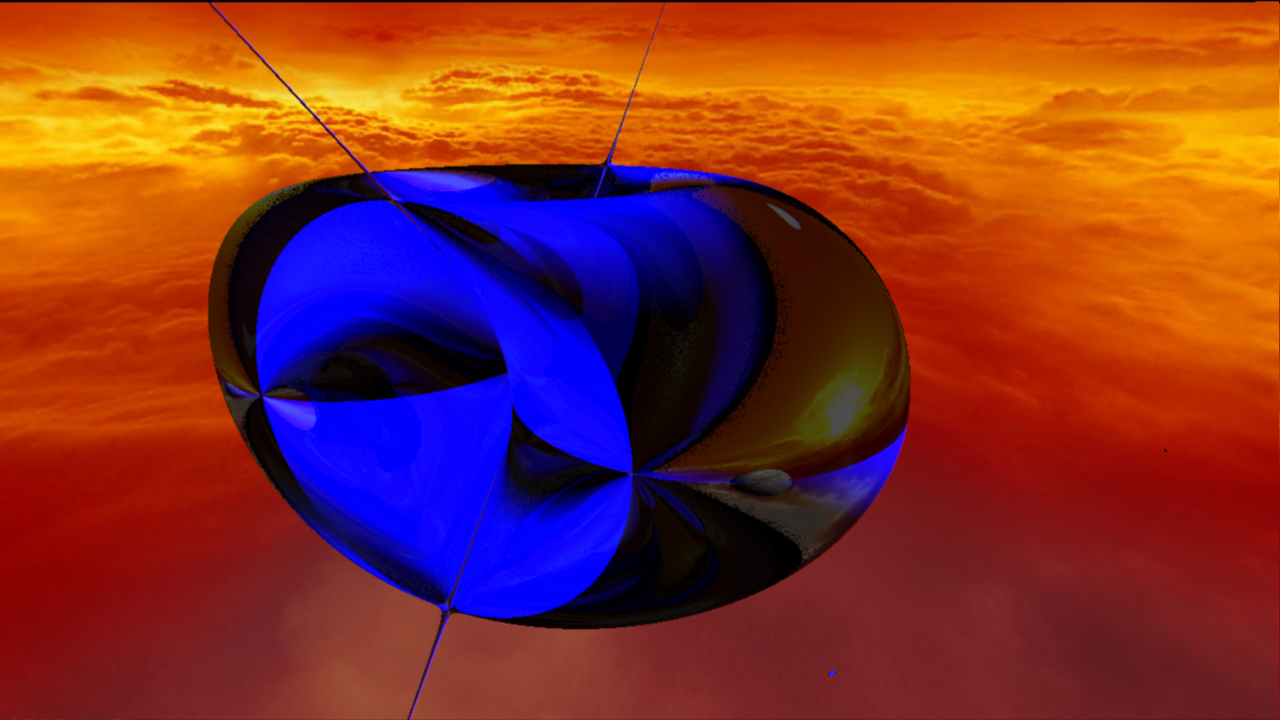
\includegraphics[width=9cm]{./imgs/bohemian_dome.png}}
	\only<19>{\textit{Bohemian Star}~:\\\bigskip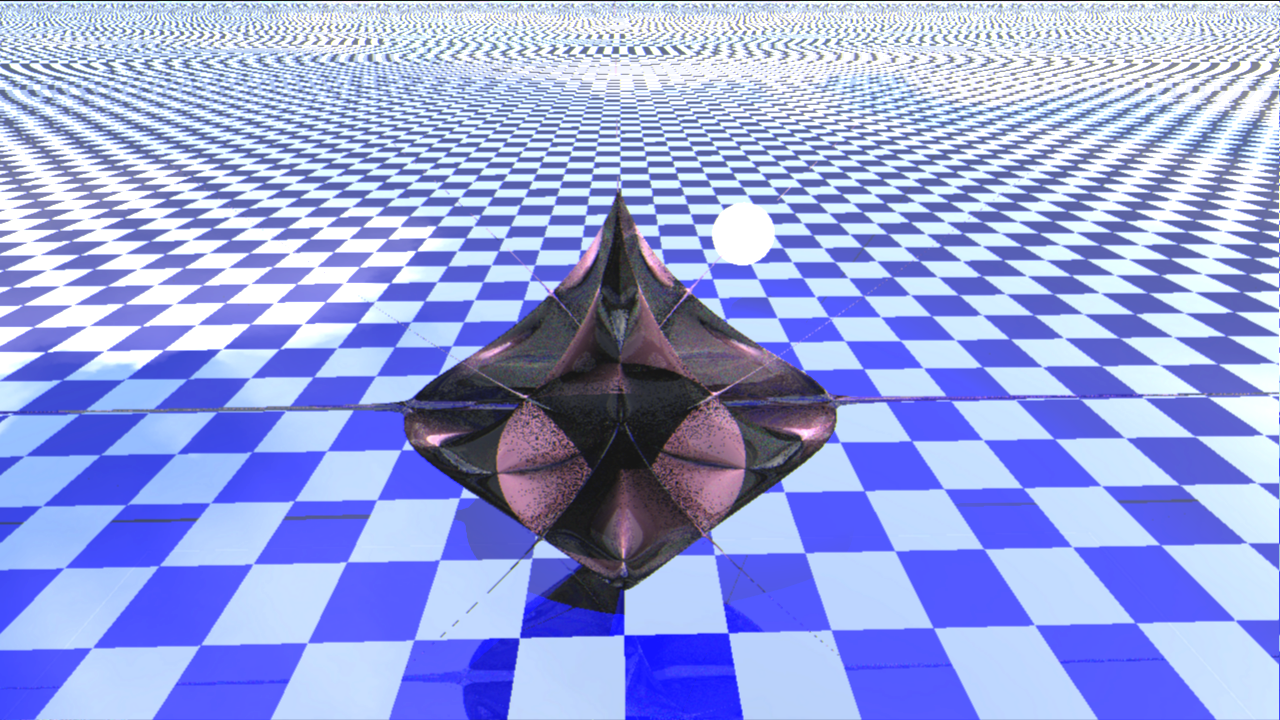
\includegraphics[width=9cm]{./imgs/bohemian_star.png}}
	\only<20>{\textit{C8}~:\\\bigskip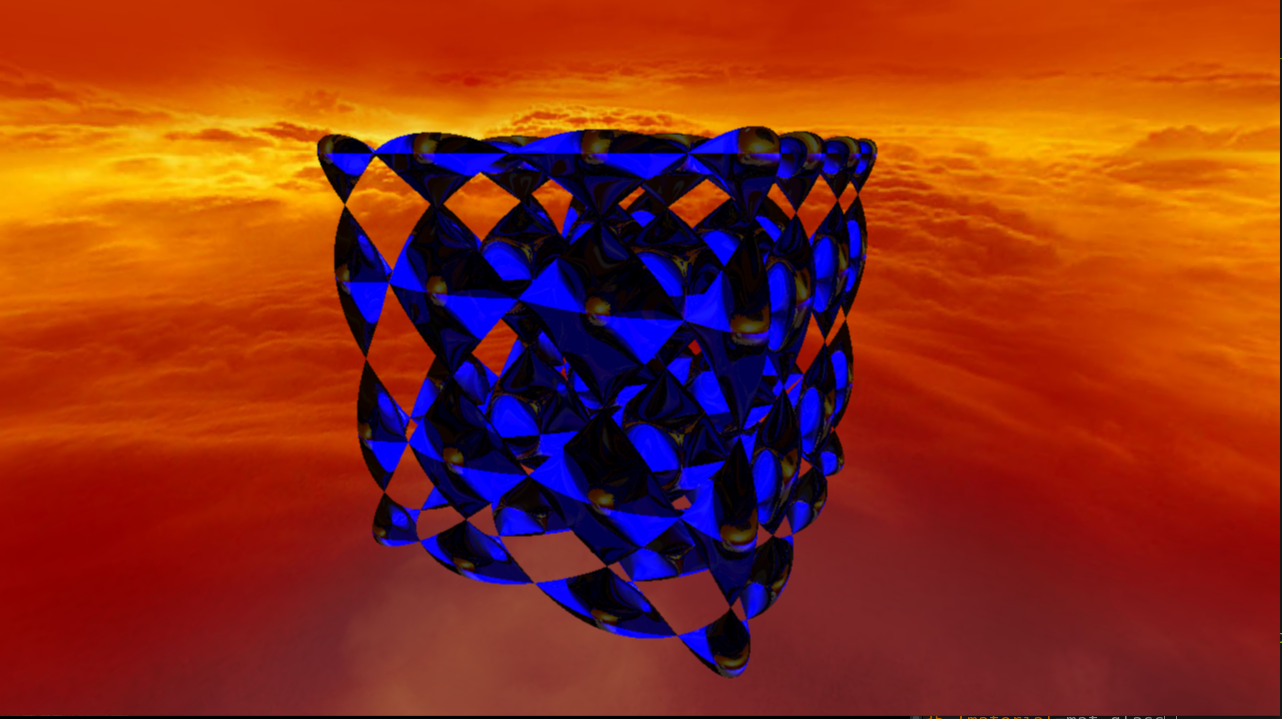
\includegraphics[width=9cm]{./imgs/c8.png}}
	\only<21>{\textit{Chubs}~:\\\bigskip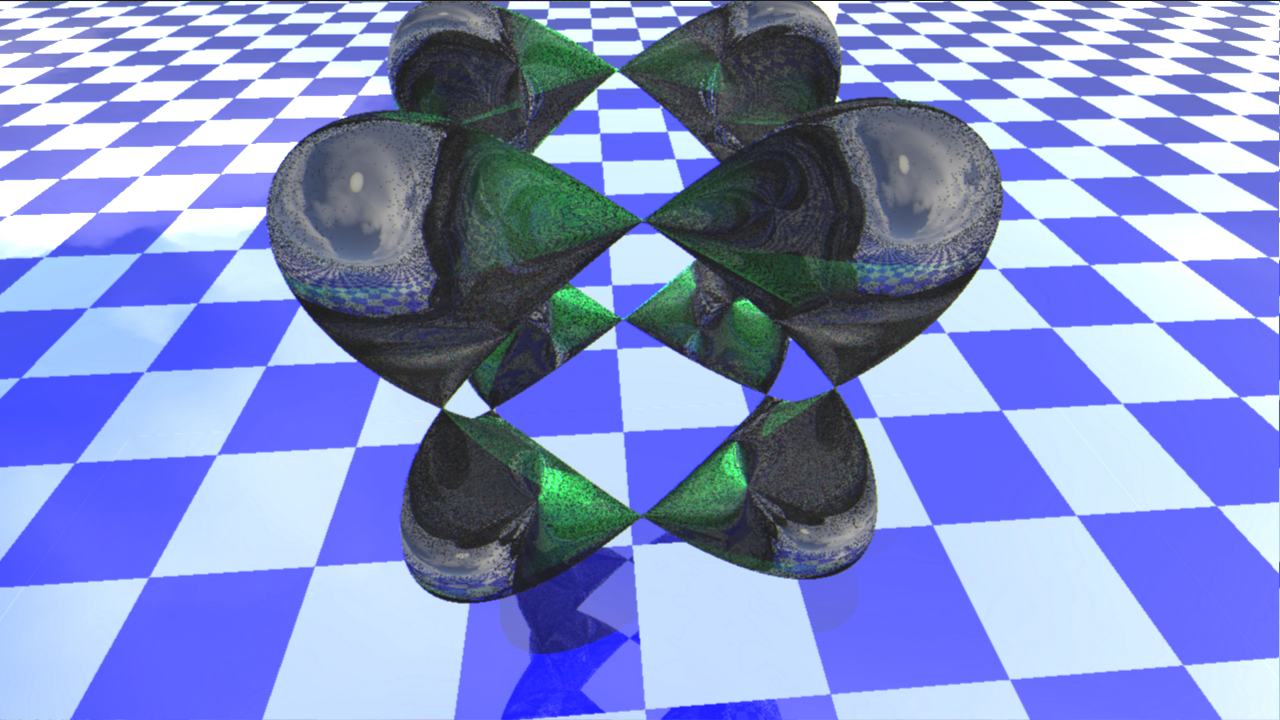
\includegraphics[width=9cm]{./imgs/chubs.png}}
	\only<22>{\textit{Quartic Cylinder}~:\\\bigskip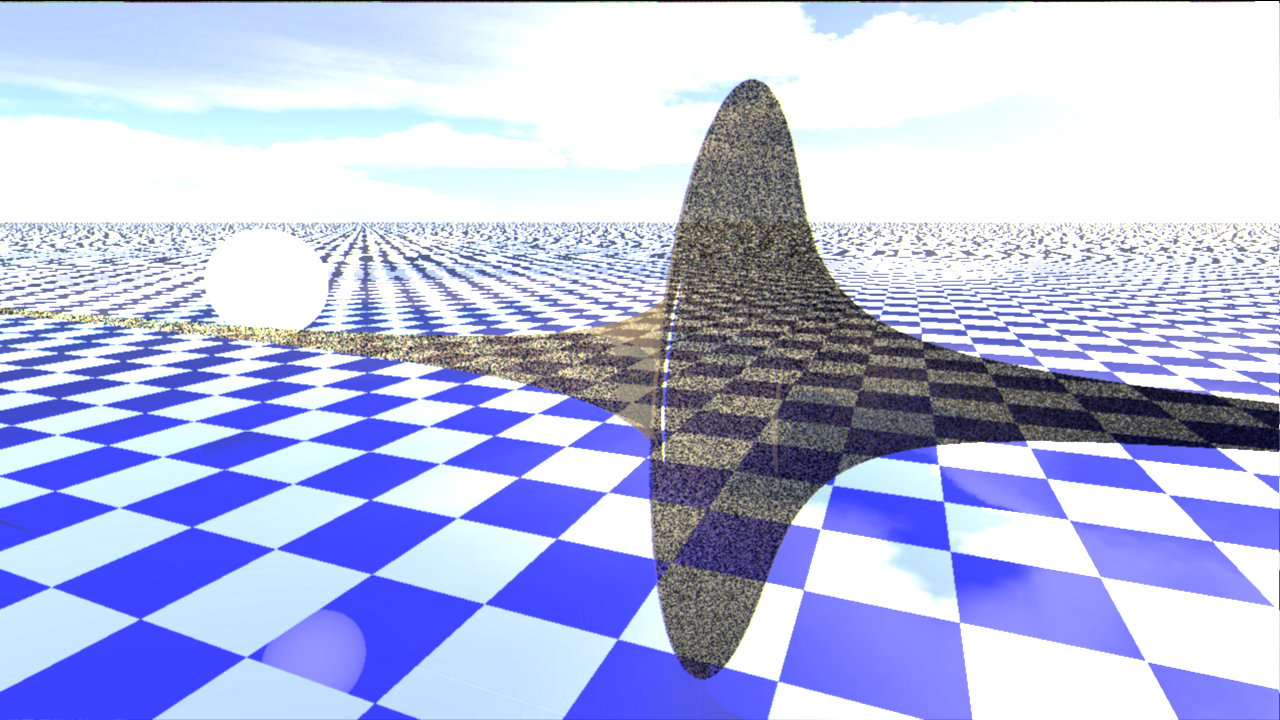
\includegraphics[width=9cm]{./imgs/quartic_cylinder.png}}
	\only<23>{\texttt{PLY}~:\\\bigskip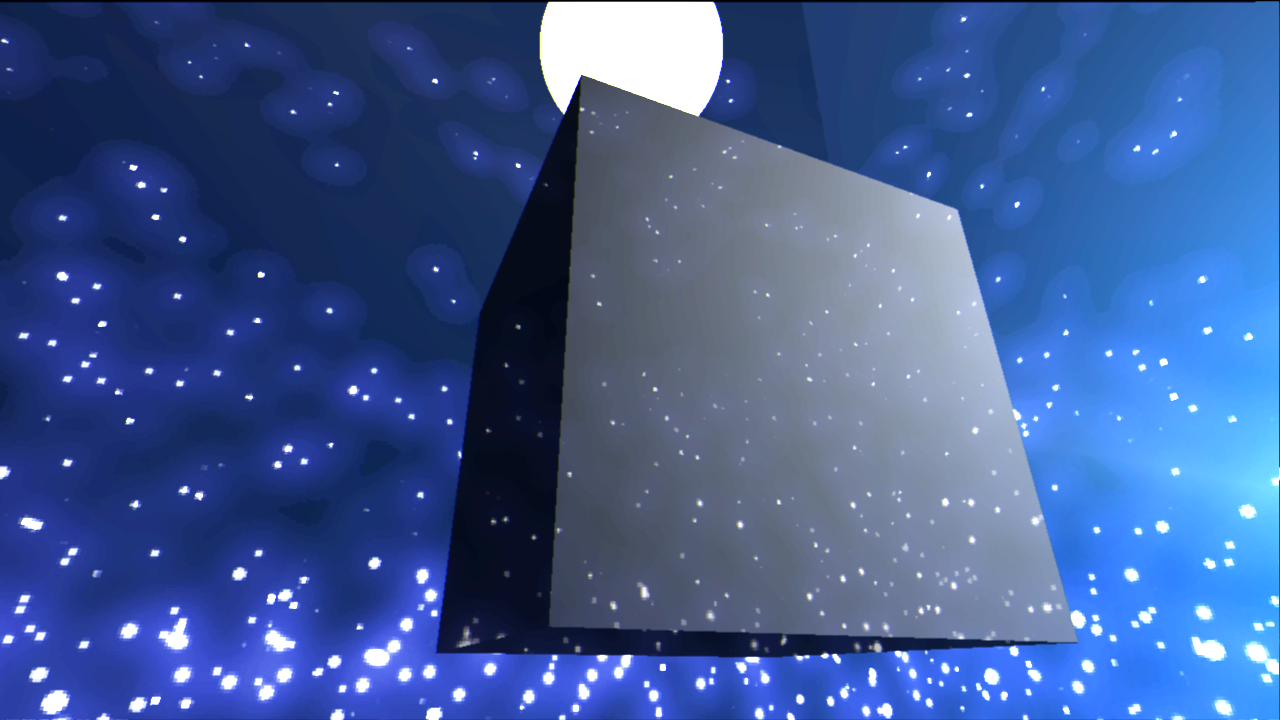
\includegraphics[width=9cm]{./imgs/cube.png}}
	\only<24>{\texttt{PLY}~:\\\bigskip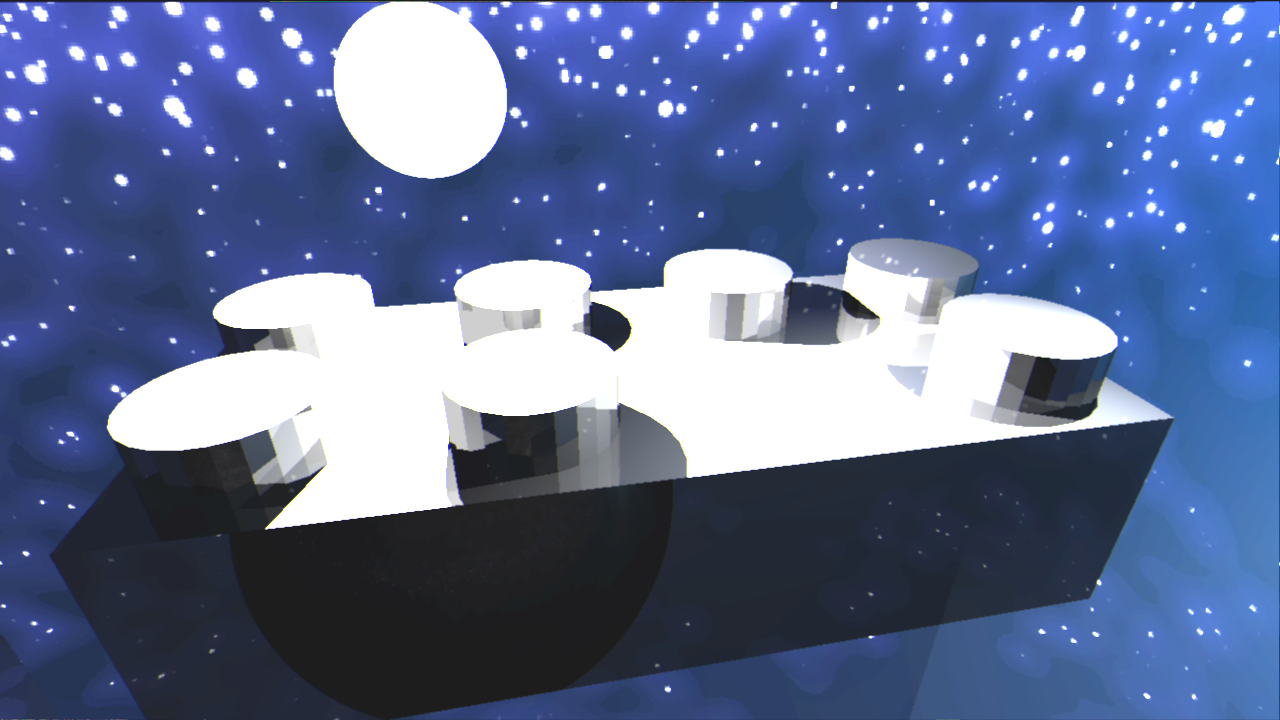
\includegraphics[width=9cm]{./imgs/lego.png}}
	\only<25>{\texttt{PLY}~:\\\bigskip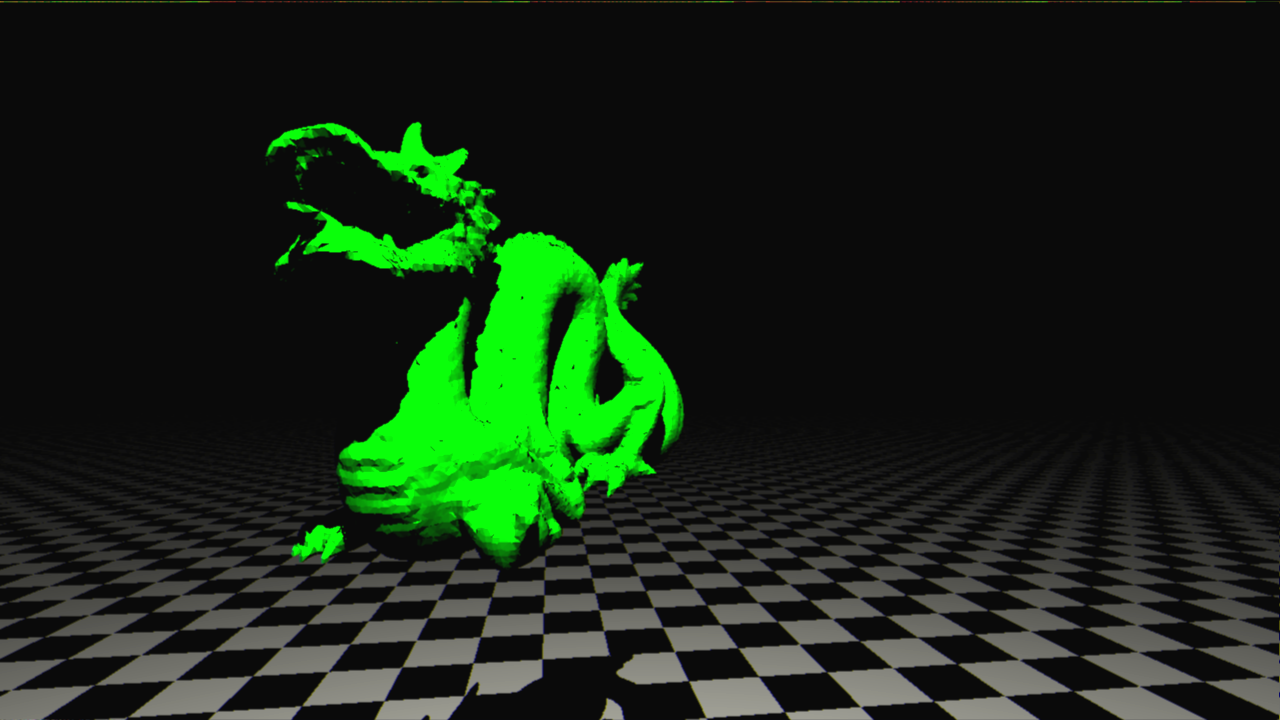
\includegraphics[width=9cm]{./imgs/dragon.png}}
	\only<26>{\texttt{PLY}~:\\\bigskip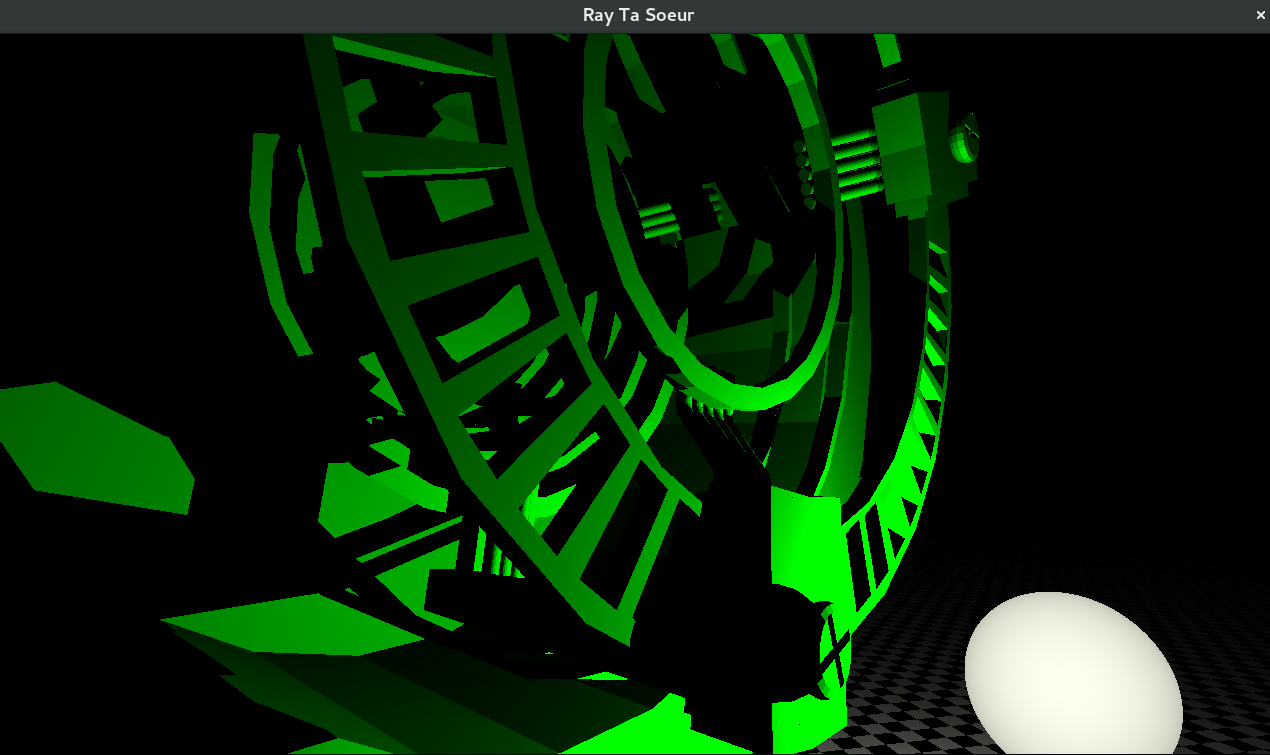
\includegraphics[width=9cm]{./imgs/ark_reactor.png}}
\end{frame}

\subsection{\texttt{PLY}}

\begin{frame}[fragile]{Gestion des \texttt{PLY}}
	\begin{block}{}
		\texttt{ply}\\\bigskip
		\texttt{format ascii 1.0\\
		format binary\_little\_endian 1.0\\
		format binary\_big\_endian 1.0}\\\bigskip
		\texttt{element vertex 12\\
		property float x\\
		property float y\\
		property float z}\\\bigskip
		\texttt{element face 10\\
		property list uchar int vertex\_indices}\\\bigskip
		\texttt{end header}\\\bigskip
	\end{block}
\end{frame}

\begin{frame}[fragile]{Gestion des \texttt{PLY}}
	\begin{center}
		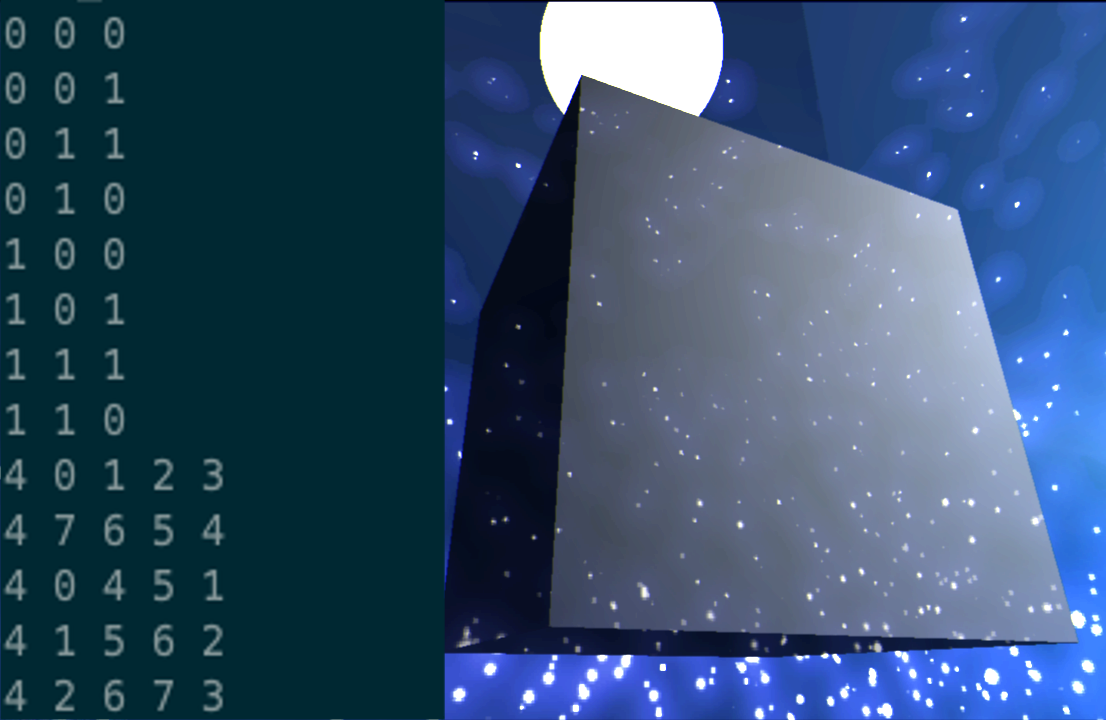
\includegraphics[width=9cm]{./imgs/cube-ply.png}
	\end{center}
\end{frame}

\begin{frame}[fragile]{Puissance des \texttt{PLY}}
	\only<1>{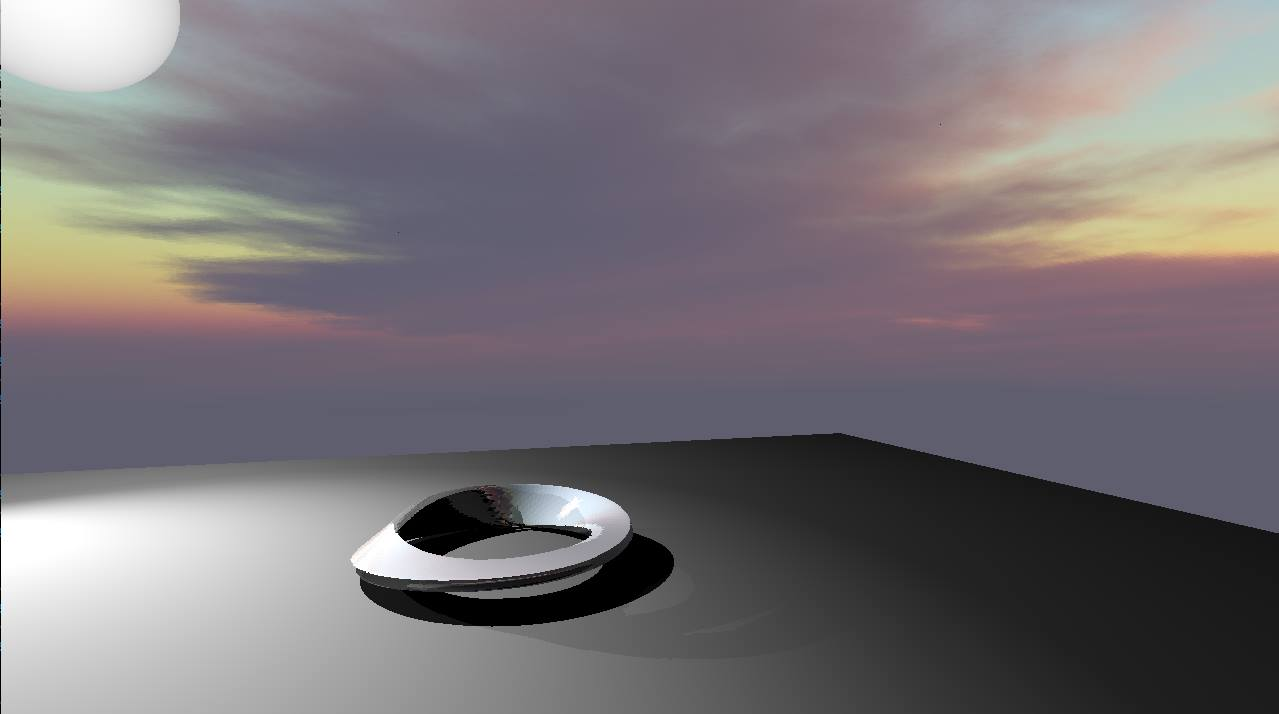
\includegraphics[width=9cm]{./imgs/ply-5.png}}
	\only<2>{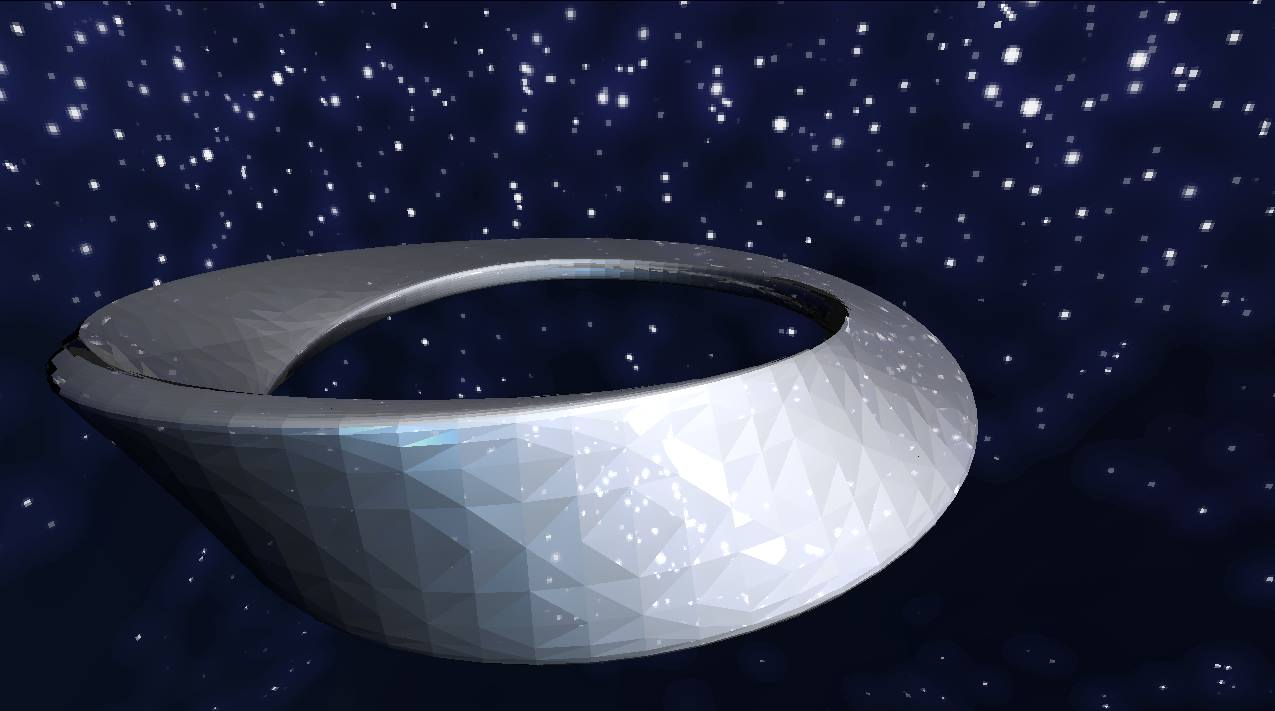
\includegraphics[width=9cm]{./imgs/ply-2.png}}
	\only<3>{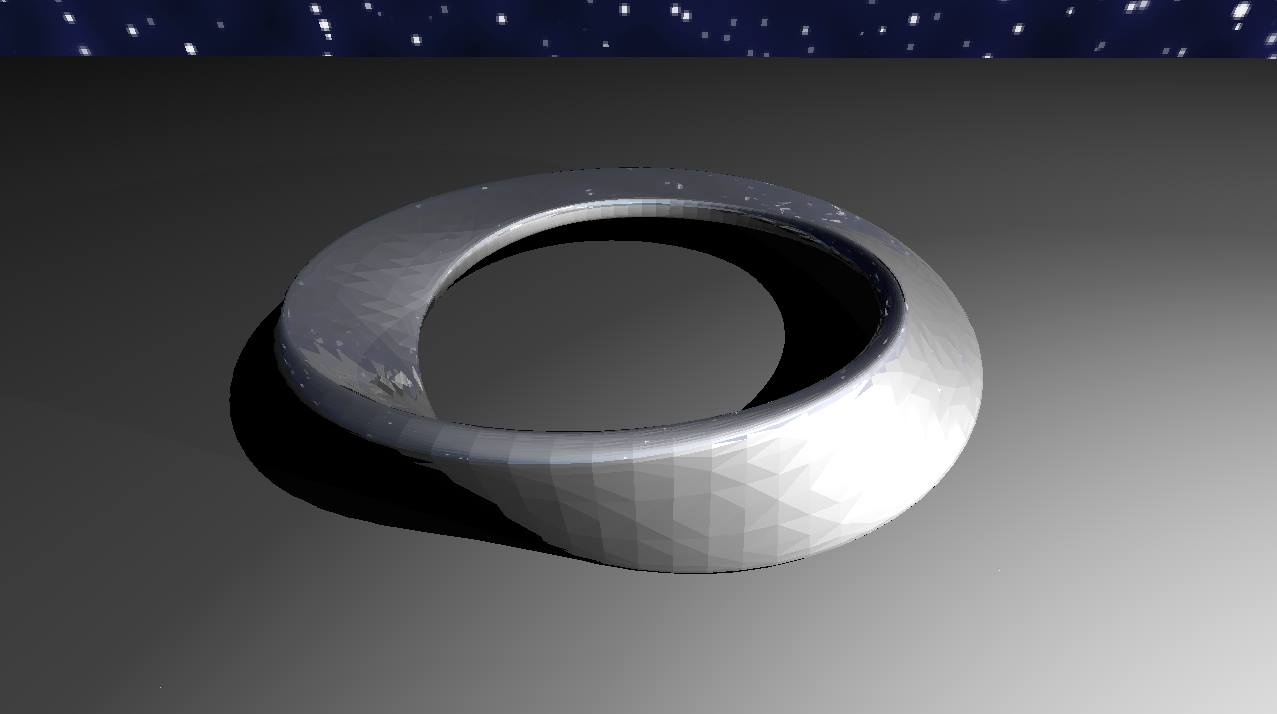
\includegraphics[width=9cm]{./imgs/ply-3.png}}
	\only<4>{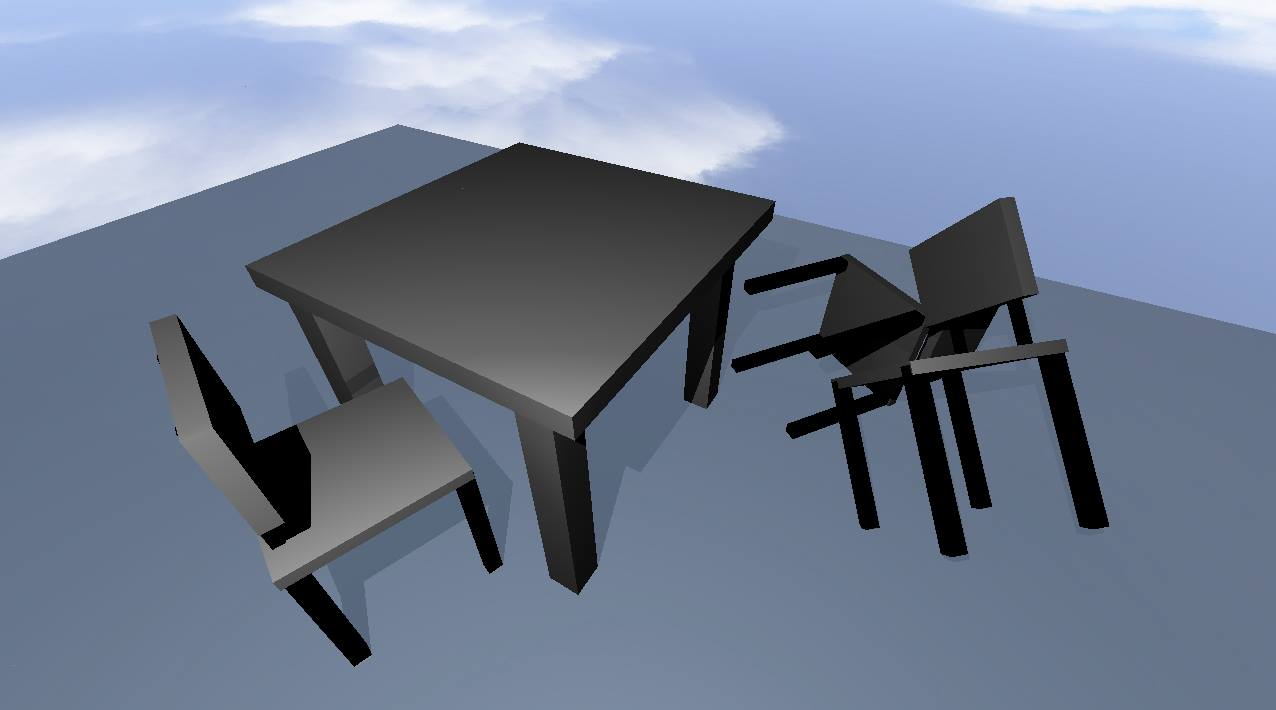
\includegraphics[width=9cm]{./imgs/ply-1.png}}
	\only<5>{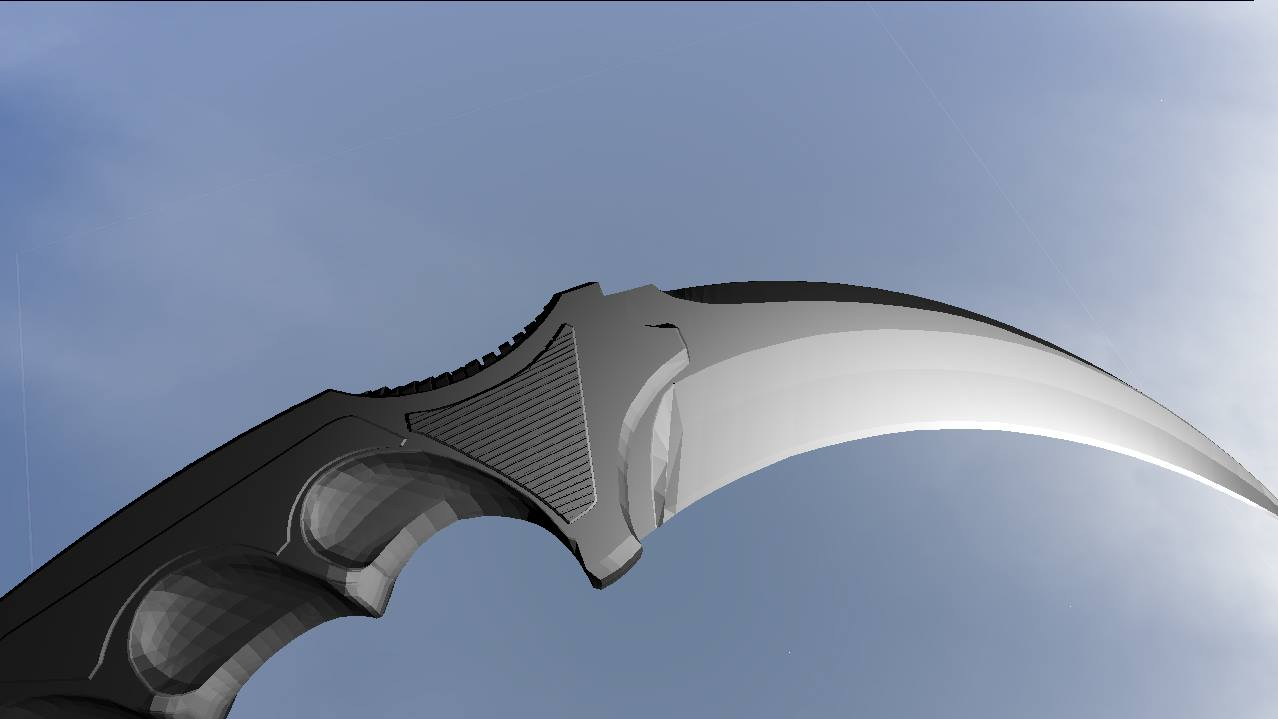
\includegraphics[width=9cm]{./imgs/ply-4.png}}
\end{frame}

\section{Effets}

\begin{frame}[fragile,t]{Effets}
	\pause
	Les effets sont appliqués sur le rendu final complet, selon différents algorithmes.

	\only<3>{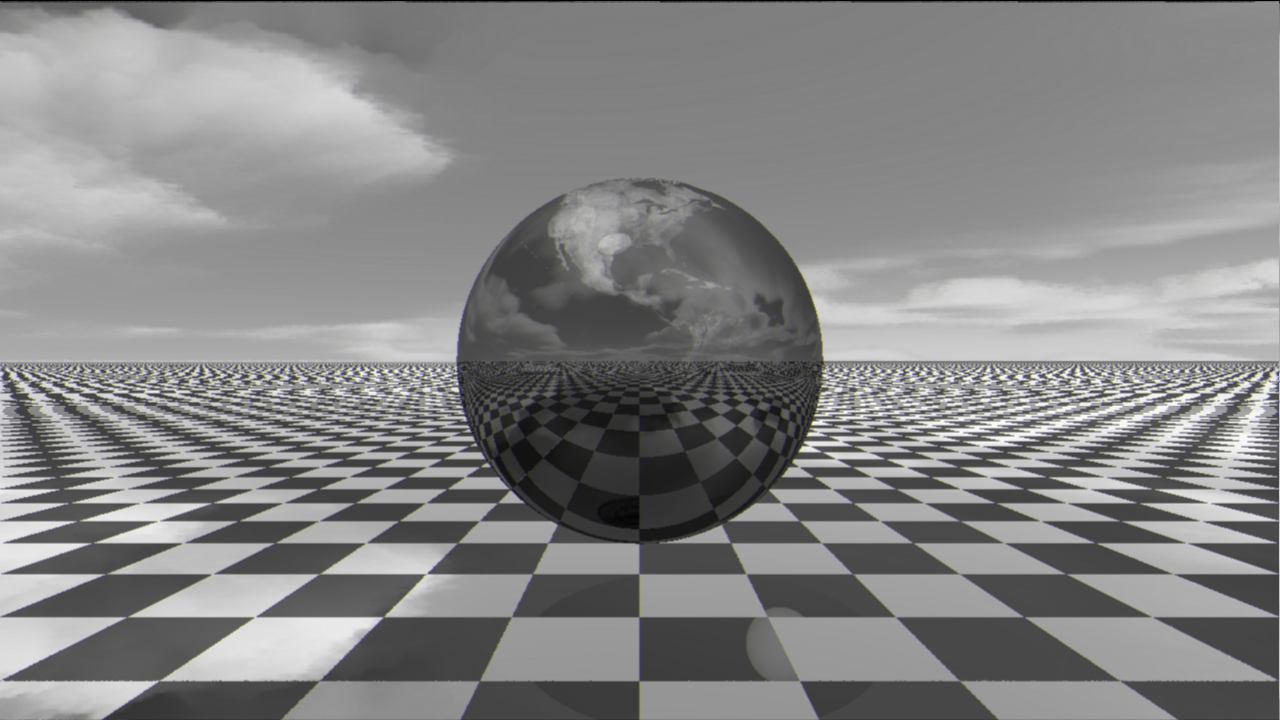
\includegraphics[width=9cm]{./imgs/black_and_white.png}}
	\only<4>{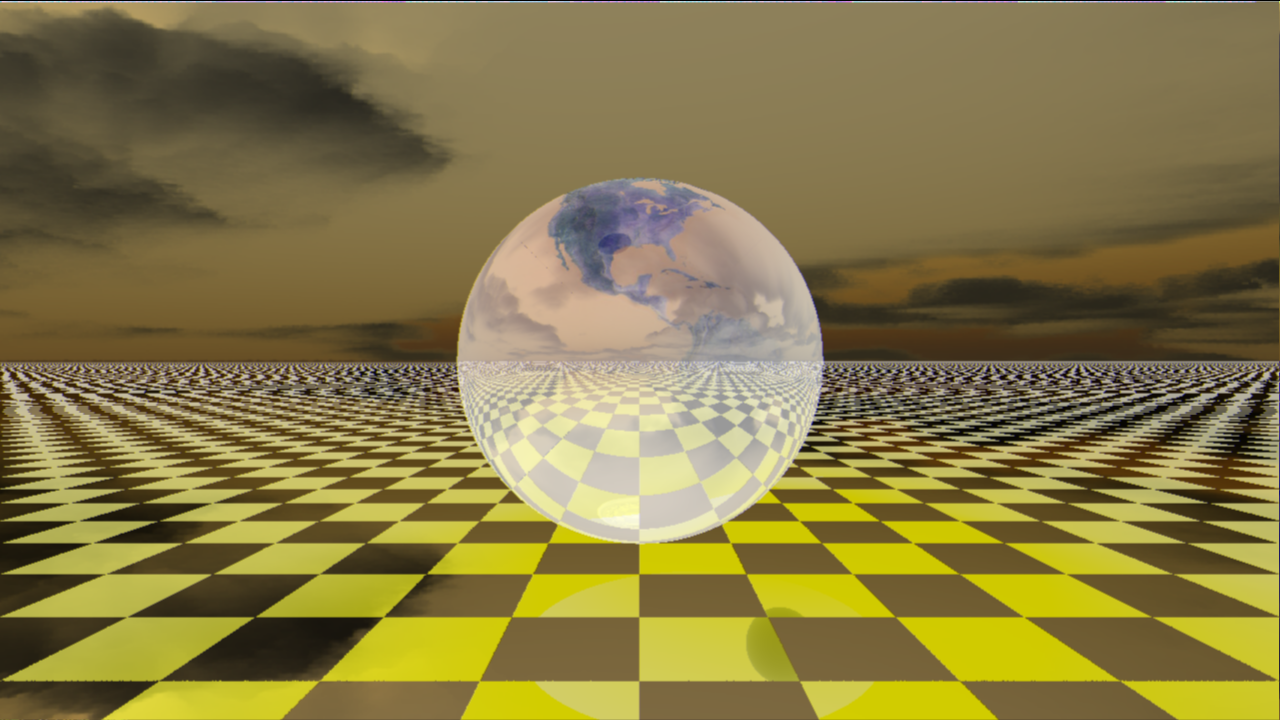
\includegraphics[width=9cm]{./imgs/negative.png}}
	\only<5>{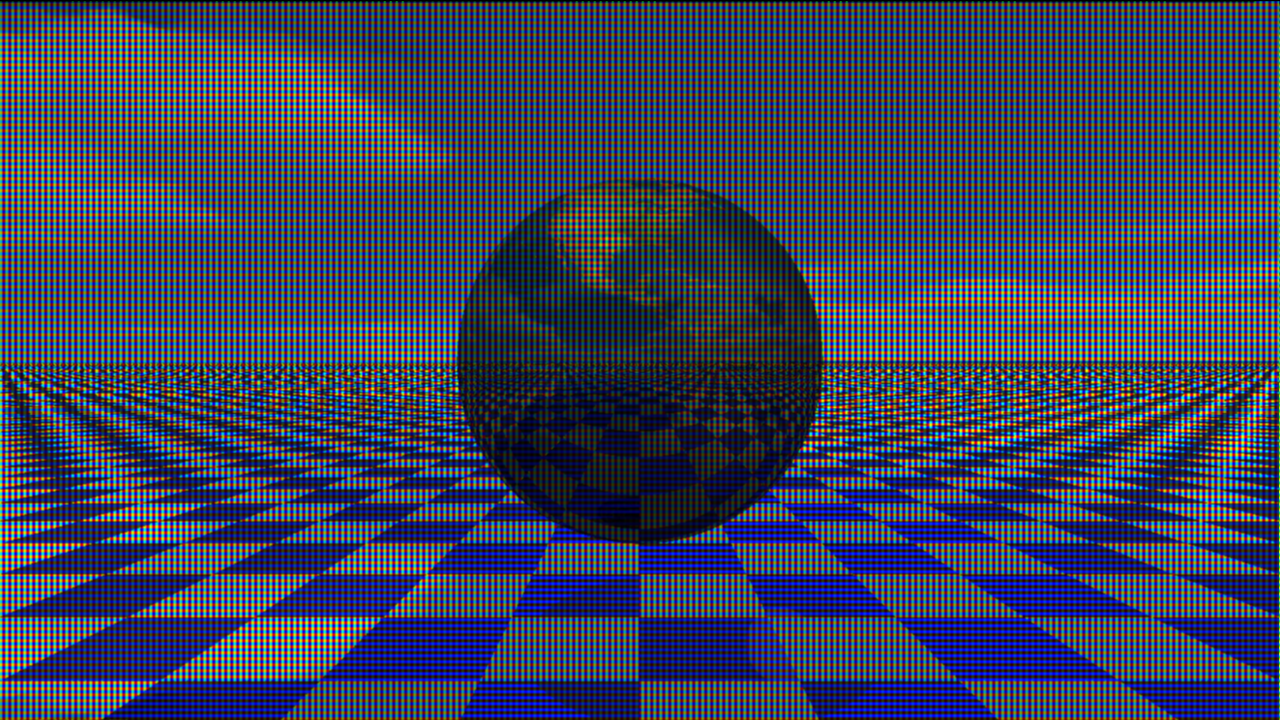
\includegraphics[width=9cm]{./imgs/bayer.png}}
	\only<6>{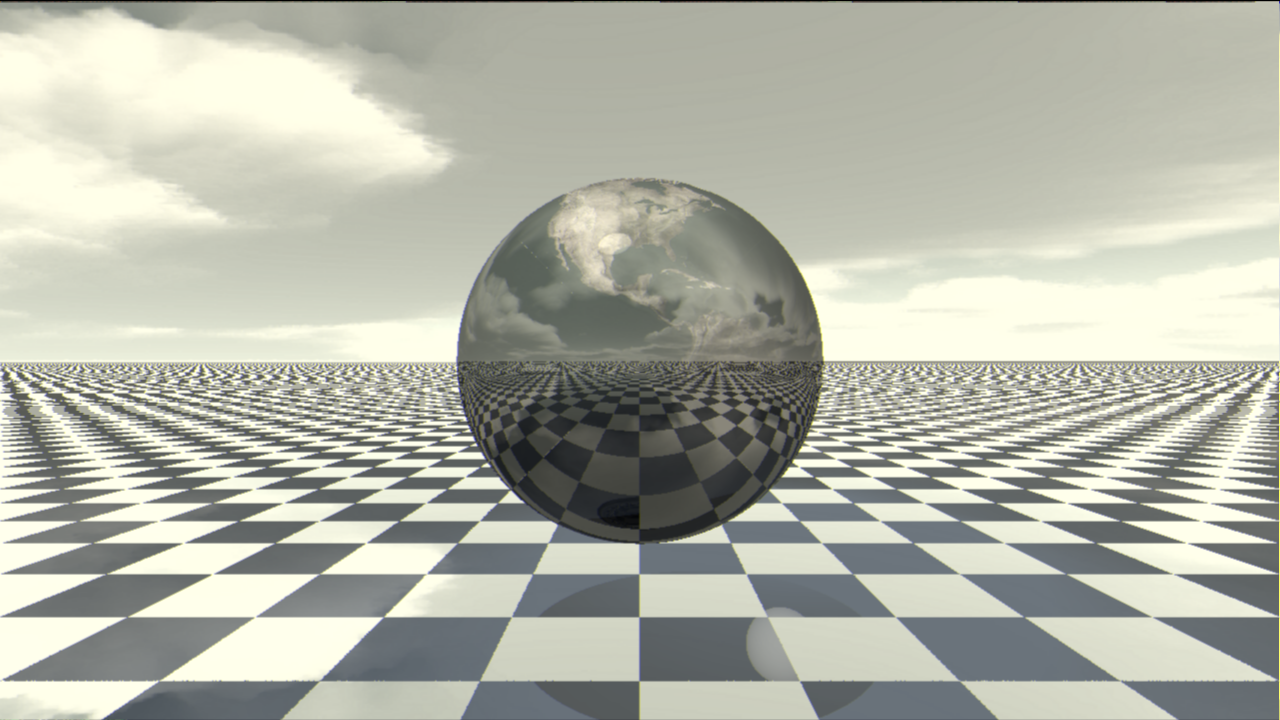
\includegraphics[width=9cm]{./imgs/sepia.png}}
\end{frame}

\section{Images}

\begin{frame}[fragile]{Un futur...~?}
	\only<1>{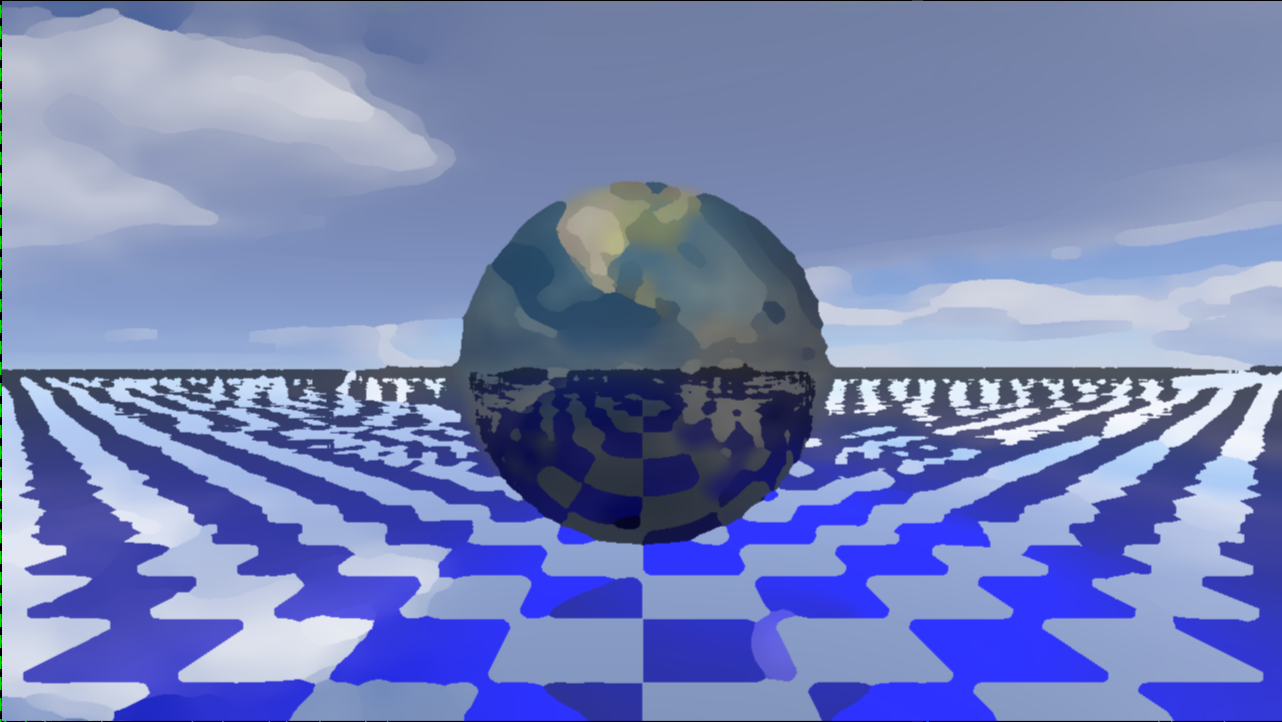
\includegraphics[width=9cm]{./imgs/pastel.png}}
	\only<2>{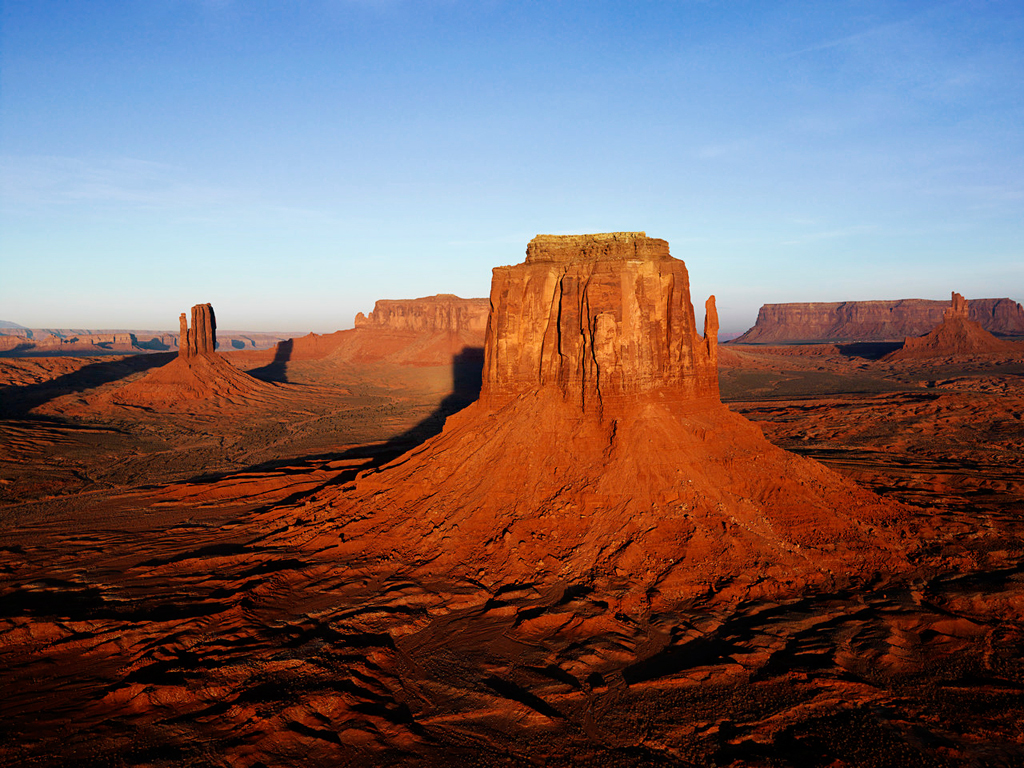
\includegraphics[width=9cm]{./imgs/stained-glass0.png}}
	\only<3>{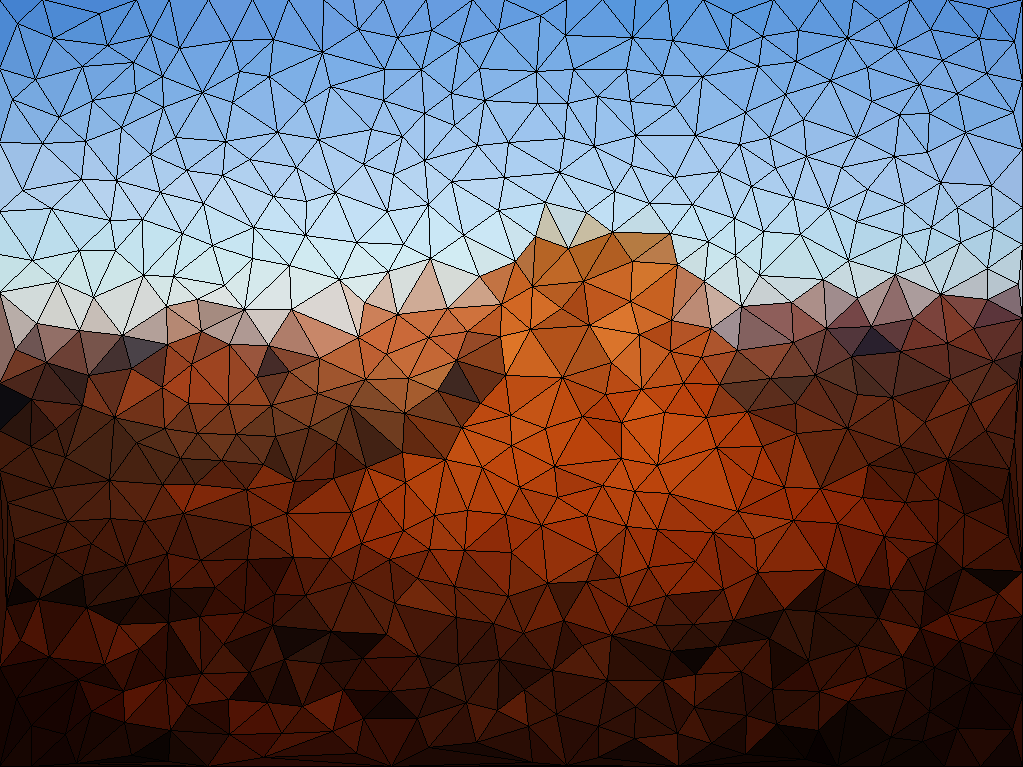
\includegraphics[width=9cm]{./imgs/stained-glass1.png}}
	\only<4>{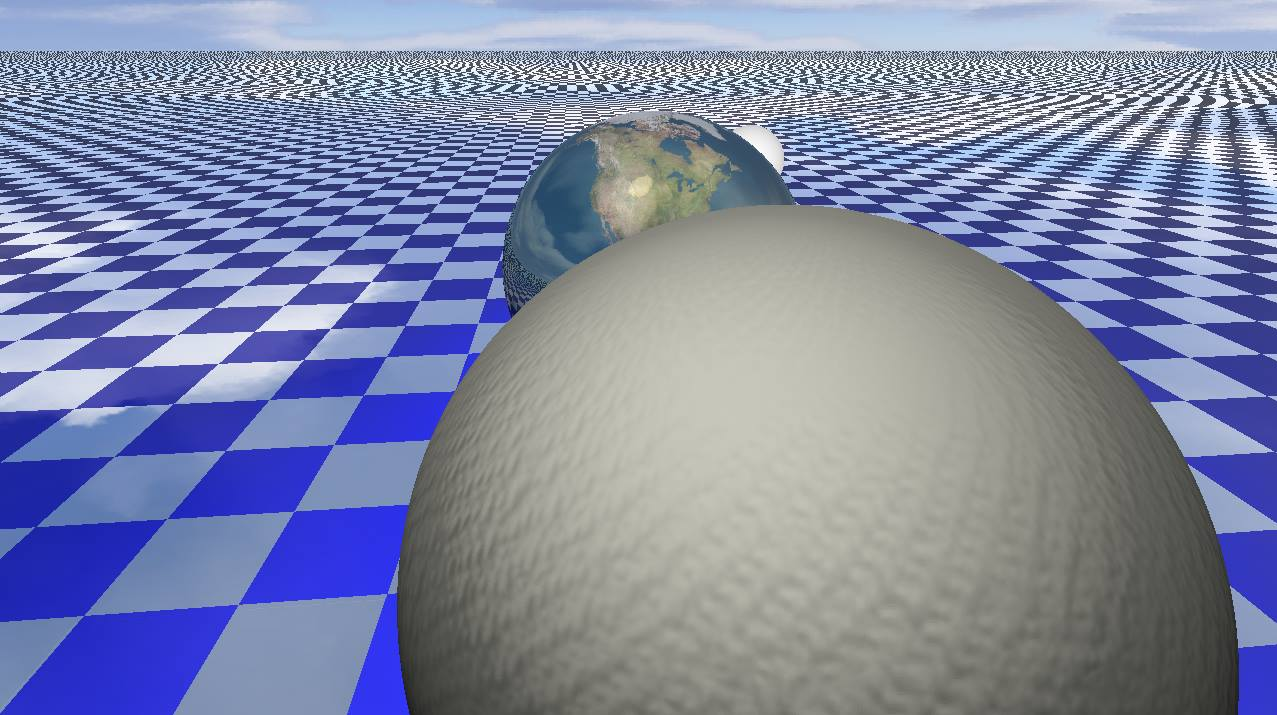
\includegraphics[width=9cm]{./imgs/bump-mapping1.png}}
	\only<5>{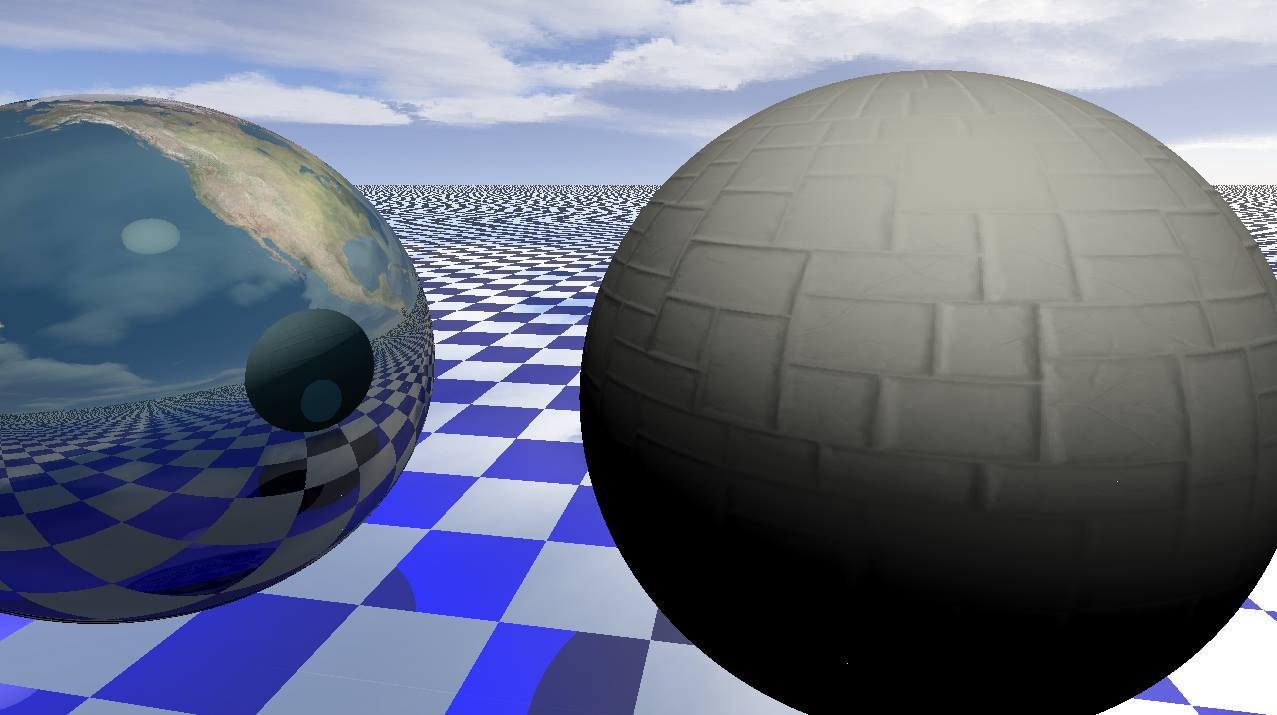
\includegraphics[width=9cm]{./imgs/bump-mapping0.png}}
\end{frame}


\plain{Questions\\{\scriptsize Merci de votre attention}}

\end{document}
